\chapter{Plataforma Web}
\section{Aplicación Web}
Se desarrollo una aplicación web mediante Vue3, FastAPI y PostgreSQL que permite al usuario subir sus archivos de secuenciación y metadata. 
Con esto el usuario puede abstraerse de tener conocimiento en línea de comando o ejecución de heramientas bioinformaticas y/o flujos de trabajo, 
ya que mediante la interfaz web el usuario solo debe seleccionar los análisis que desea realizar.
La información ingresada por el usuario es guardada en la base de datos y mediante un script se generan los parámetros necesarios para la ejecución del flujo de trabajo.
Una vez el pipeline termina de ejecutarse se escriben los resultados en la base de datos. 
La plataforma lee esta información directa de la base de datos y despliega los resultados en forma de tablas y gráficos en la sección de análisis.


A continuación se detalla cada una de las vistas de la aplicación web y su funcionalidad.
% \subsection{Middleware}
% \subsection{Security}

\subsection{Login}
Al ingresar en la página de Login, el usuario deberá ingresar su nombre de usuario y contraseña.
En caso de que los datos sean correctos será redireccionado a la página de proyectos (Ver sección \ref{projects}).
En caso de que los datos sean incorrectos se mostrará un mensaje de error \textit{“Usuario o contraseña incorrectos”} y deberá ingresar sus credenciales nuevamente.


\begin{figure}[ht]
    \centering
    \begin{subfigure}[b]{0.45\textwidth}
        \centering
        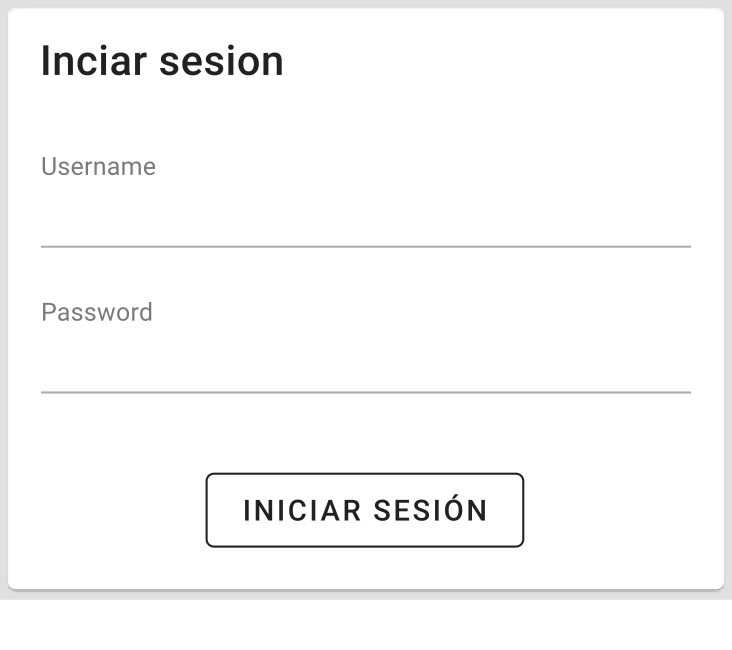
\includegraphics[width=\textwidth]{images/app/login.png}
        \caption{Vista de inicio de sesión por defecto \newline}
        \label{fig:app-login_default}
    \end{subfigure}
    \hfill
    \begin{subfigure}[b]{0.45\textwidth}
        \centering
        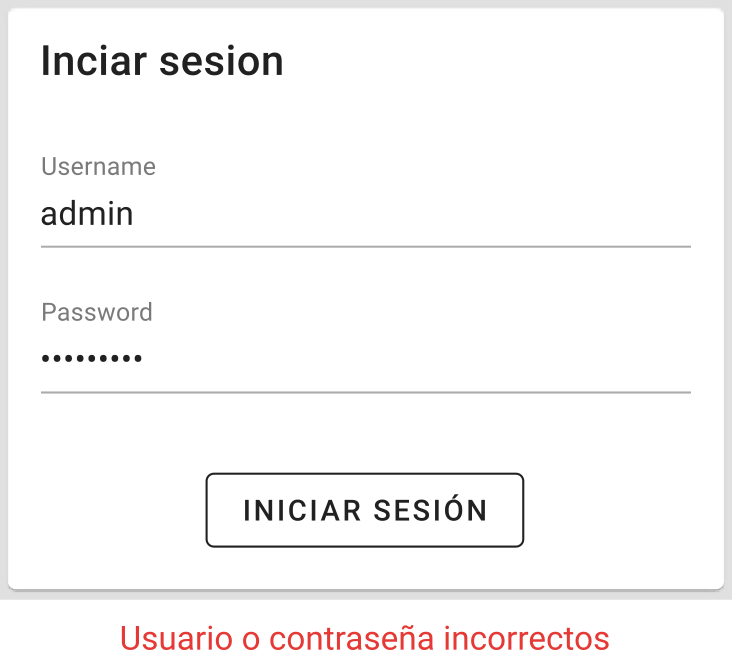
\includegraphics[width=\textwidth]{images/app/login-error.png}
        \caption{Vista de inicio de sesión con mensaje de error al ingresar credenciales inválidas}
        \label{fig:app-login_error}
    \end{subfigure}
    \caption{Vista de Inicio de sesión}
    \label{fig:app-login}
\end{figure}

% \hl{Registrarse - vista}
\subsection{Navbar}
Una vez que el usuario inicia sesión, va a poder visualizar la barra de navegación de la plataforma en la parte superior de la página. 
% La plataforma cuenta con las siguientes secciones en la barra de navegación:
% \begin{itemize}
%     \item \textit{Results}
%     \item \textit{New analyses}
%     \item \textit{Change password}: Cambiar contraseña
%     \item \textit{Log out}: Cerrar sesión en la plataforma
% \end{itemize}
\begin{figure}[H]
    
\includegraphics[width=1\linewidth]{images/app/navbar.png}
    \caption{Barra de navegación}
    \label{fig:app-nabvar}
\end{figure}

A continuación se describen las funcionalidades de cada una de las secciones de la barra de navegación:

\subsection{Cambio de contraseña}
Una vez que el usuario validó sus credenciales va a poder acceder a la vista de cambio de contraseña a través de la barra de navegación (Figura~\ref{fig:app-change-psw_default}).



Para realizar el cambio de contraseña, deberá ingresar su contraseña actual y su nueva contraseña dos veces.
En caso de que la contraseña sea cambiada con éxito se mostrará el mensaje \textit{“Contraseña cambiada con exito“} (Figura~\ref{fig:app-change-psw-success}).


\begin{figure}[H]
    \centering
    \begin{subfigure}[b]{0.45\textwidth}
        \centering
        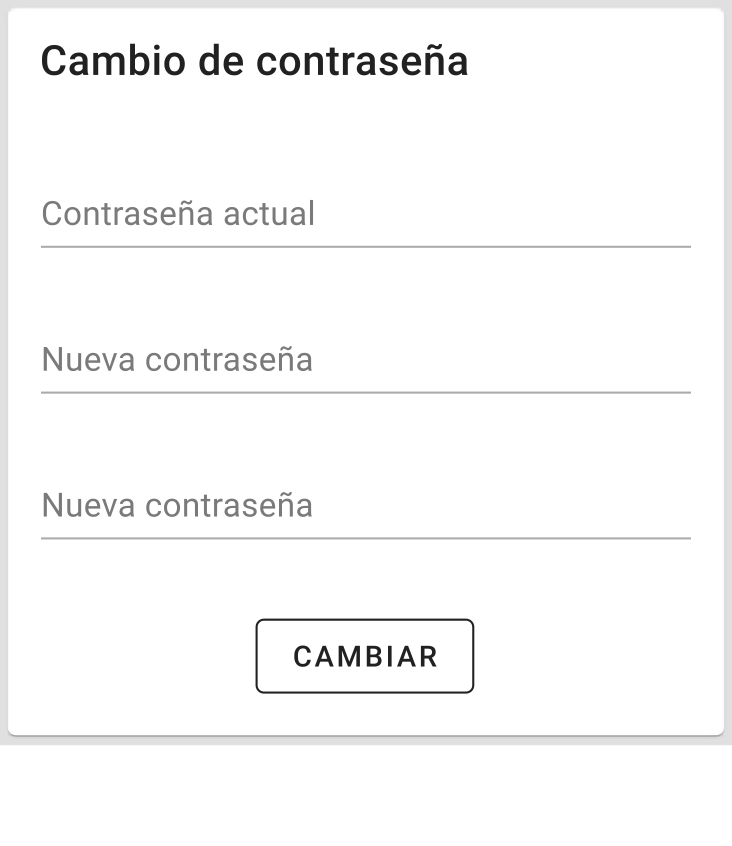
\includegraphics[width=\textwidth]{images/app/change-psw-def.png}
        \caption{Vista de cambio de contraseña por defecto \newline}
        \label{fig:app-change-psw_default}
    \end{subfigure}
    \hfill
    \begin{subfigure}[b]{0.45\textwidth}
        \centering
        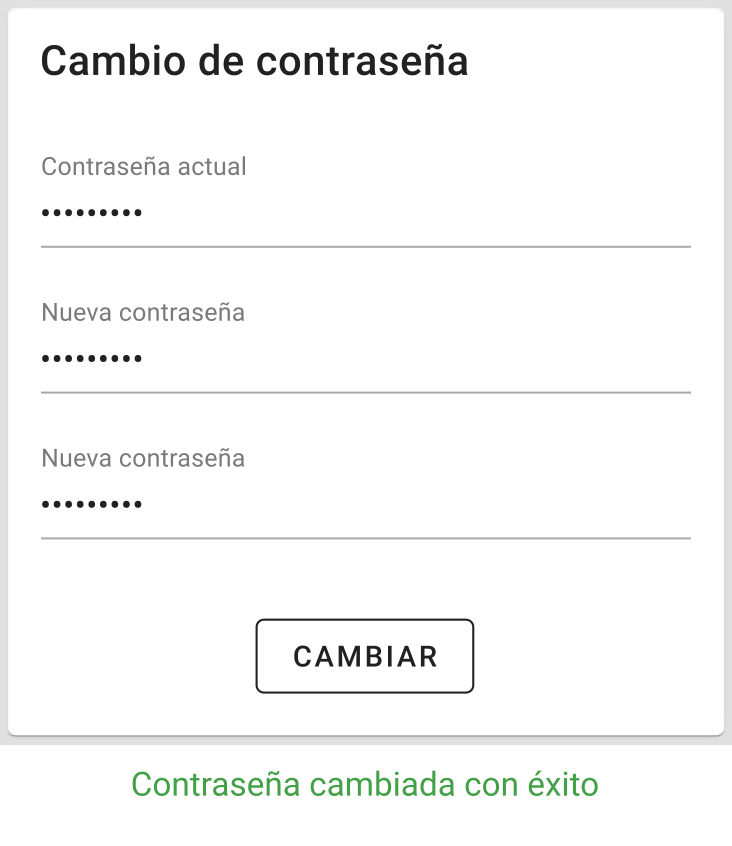
\includegraphics[width=\textwidth]{images/app/change-psw-sucess.png}
        \caption{Vista de cambio de contraseña realizado con exito}
        \label{fig:app-change-psw-success}
    \end{subfigure}
    % \caption{Vista de Cambio de contraseña (I)}
    \label{fig:app-change-psw-1}
\end{figure}
En caso de que la contraseña actual sea incorrecta se mostrará el mensaje de error  \textit{“Contraseña incorrecta”} (Figura~\ref{fig:app-change-psw_error-1}).
En caso de que las contraseñas nuevas no coincidan se mostrará el mensaje de error \textit{“Las contraseñas no coinciden”} (Figura~\ref{fig:app-change-psw_error-2})
\begin{figure}[H]
    \centering
    \begin{subfigure}[b]{0.45\textwidth}
        \centering
        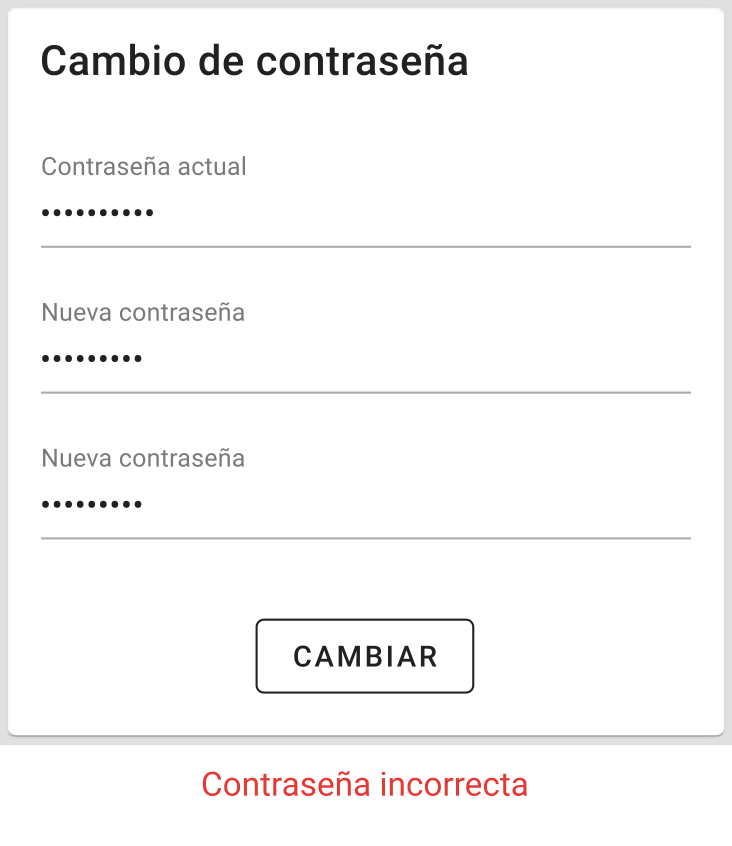
\includegraphics[width=\textwidth]{images/app/change-psw-error1.png}
        \caption{Vista de cambio de contraseña al ingresar contraseña incorrecta}
        \label{fig:app-change-psw_error-1}
    \end{subfigure}
    \hfill
    \begin{subfigure}[b]{0.45\textwidth}
        \centering
        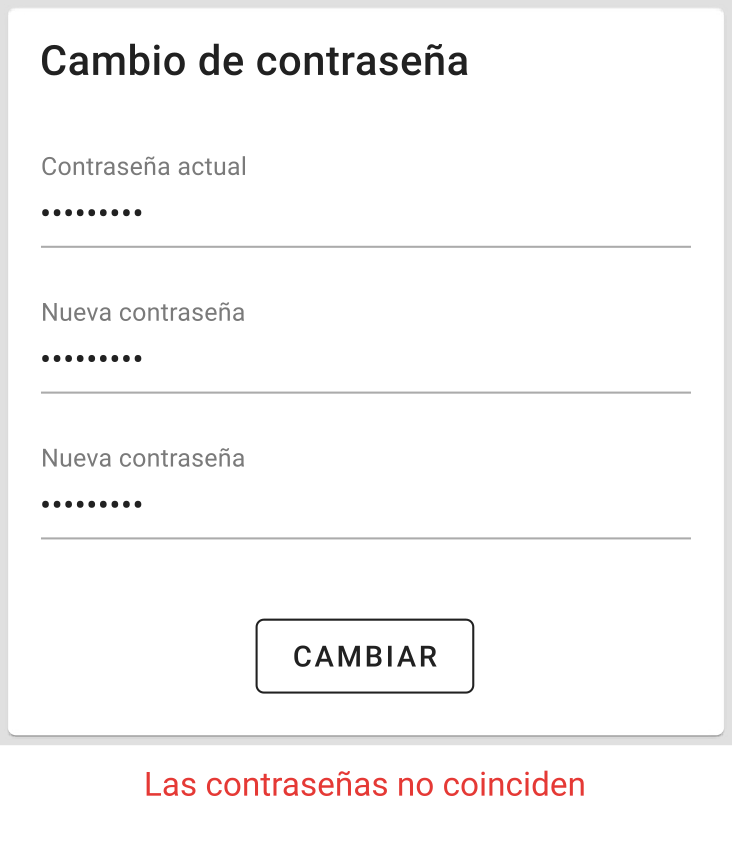
\includegraphics[width=\textwidth]{images/app/change-psw-error2.png}
        \caption{Vista de cambio de contraseña al ingresar contraseñas que no coinciden}
        \label{fig:app-change-psw_error-2}
    \end{subfigure}
    % \caption{Vista de Cambio de contraseña (II)}
    \label{fig:app-change-psw-2}
\end{figure}

En el caso de que la nueva contraseña no cumpla los críterios de seguridad (longitud mínima de 8 caracteres y al menos un número) se mostrará el mensaje de error  \textit{“La contraseña debe tener al menos 8 caracteres / La contraseña debe tener al menos un número”} (Figura~\ref{fig:app-change-psw_error-1}).
\begin{figure}[H]
    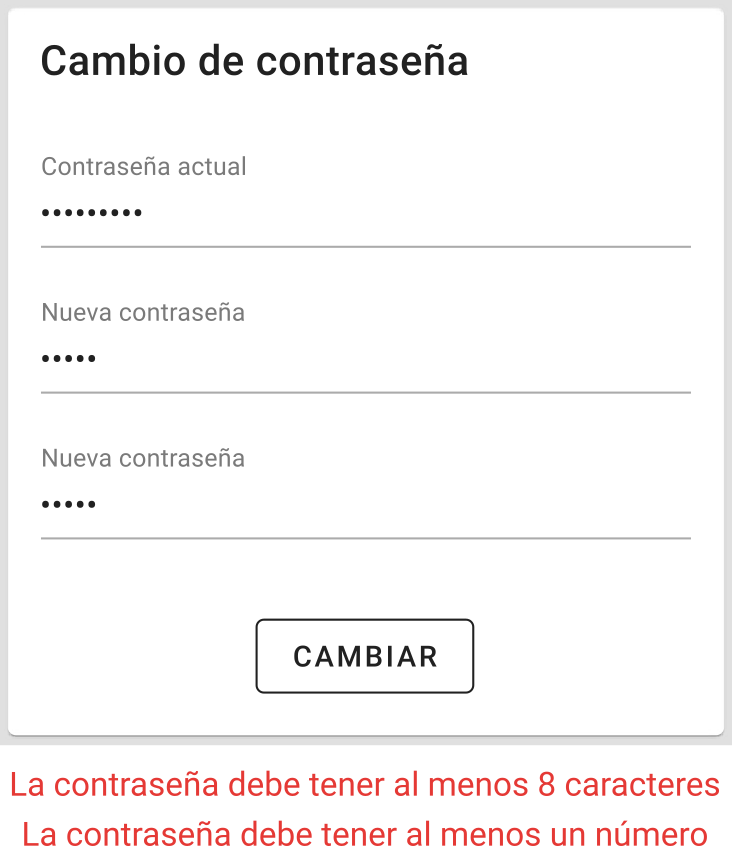
\includegraphics[width=0.45\linewidth]{images/app/change-psw-error3.png}
    \captionsetup{justification=raggedright, width=0.45\linewidth, singlelinecheck=off}

    % \captionsetup{width=0.45\linewidth}
    \caption{Vista de cambio de contraseña al ingresar una nueva contraseña que no cumple con los críterios de seguridad}
    \label{fig:app-change-psw_error-3}
\end{figure}

% \begin{figure}[H]
%     \centering
%     \begin{subfigure}[b]{0.4\textwidth}
%         \centering
%         \includegraphics[width=\textwidth]{images/app/chage-psw-def.png}
%         \caption{a}
%         \label{fig:subfig1}
%     \end{subfigure}
%     \hfill
%     \begin{subfigure}[b]{0.4\textwidth}
%         \centering
%         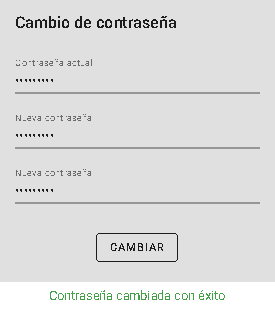
\includegraphics[width=\textwidth]{images/app/chage-psw-sucess.png}
%         \caption{b}
%         \label{fig:subfig2}
%     \end{subfigure}

%     \vskip\baselineskip

%     \begin{subfigure}[b]{0.4\textwidth}
%         \centering
%         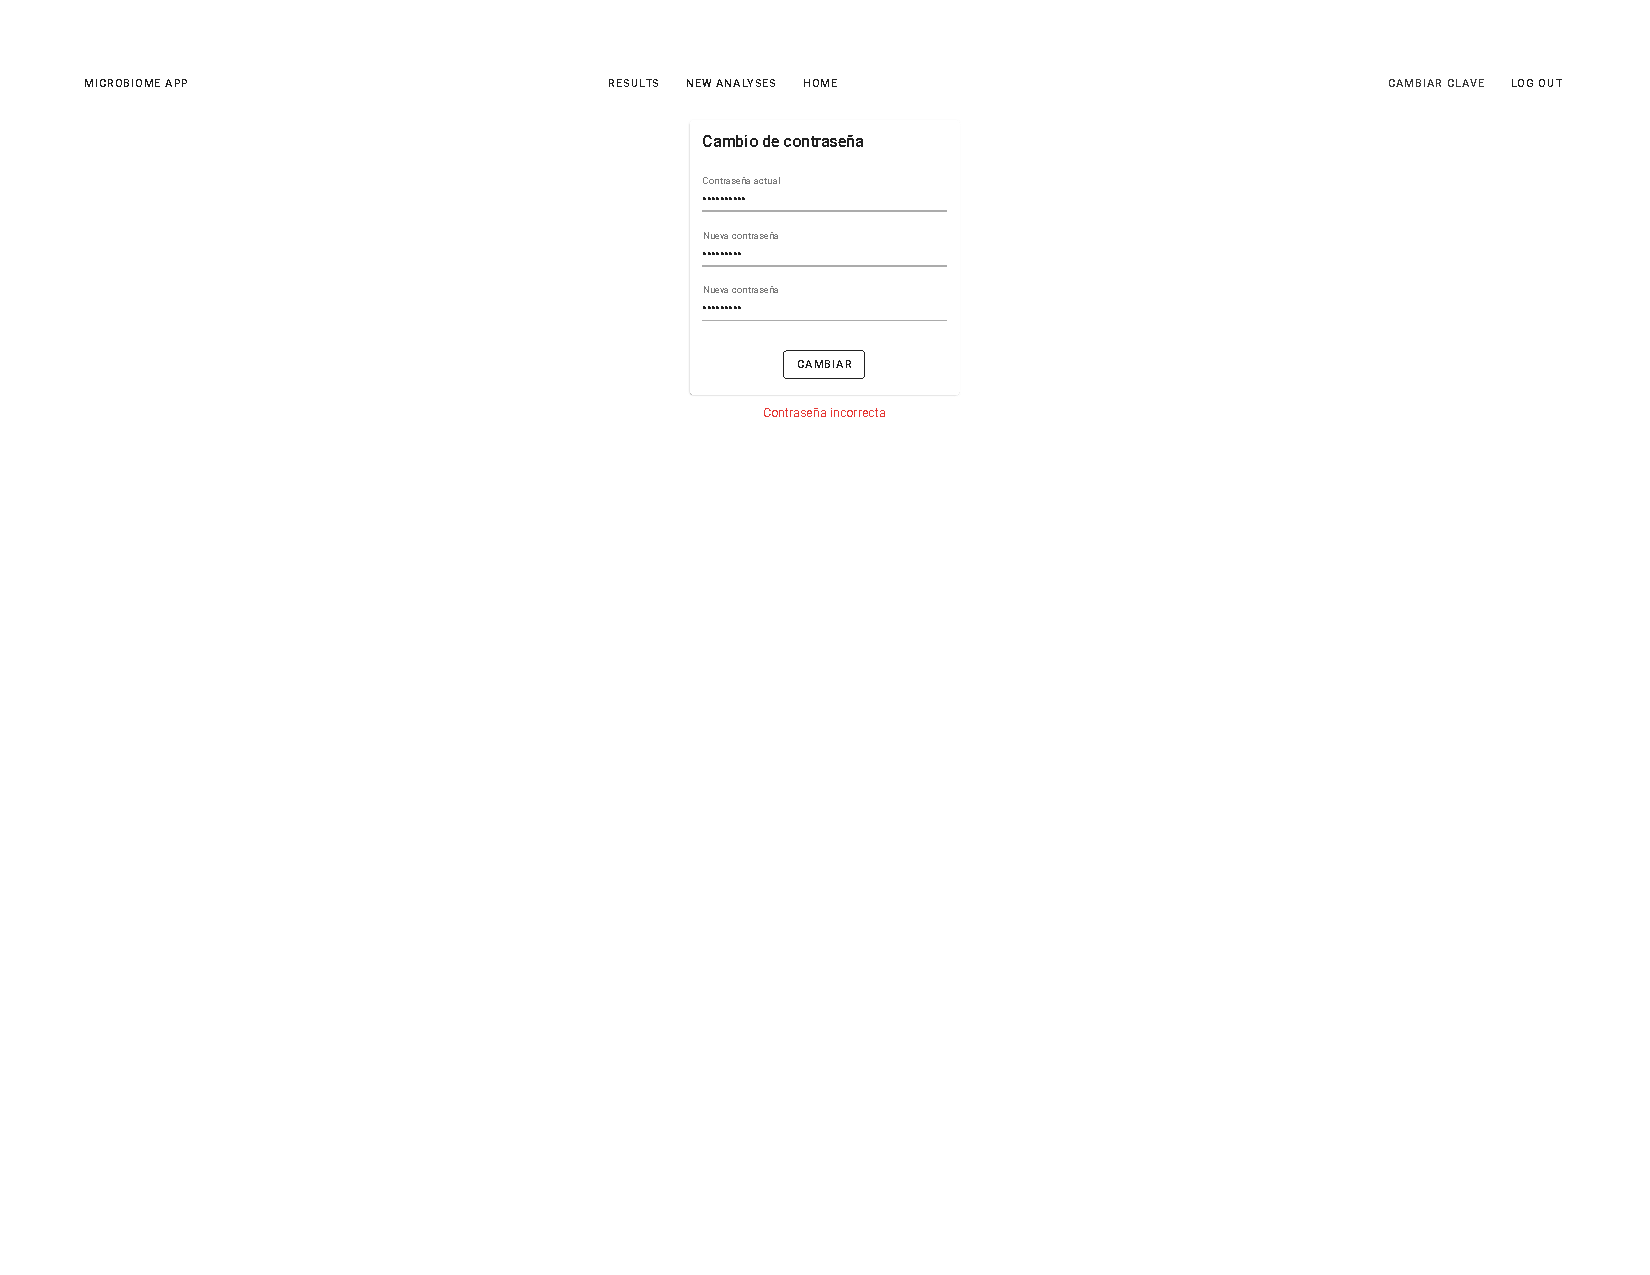
\includegraphics[width=\textwidth]{images/app/chage-psw-error1.png}
%         \caption{c}
%         \label{fig:subfig3}
%     \end{subfigure}
%     \hfill
%     \begin{subfigure}[b]{0.4\textwidth}
%         \centering
%         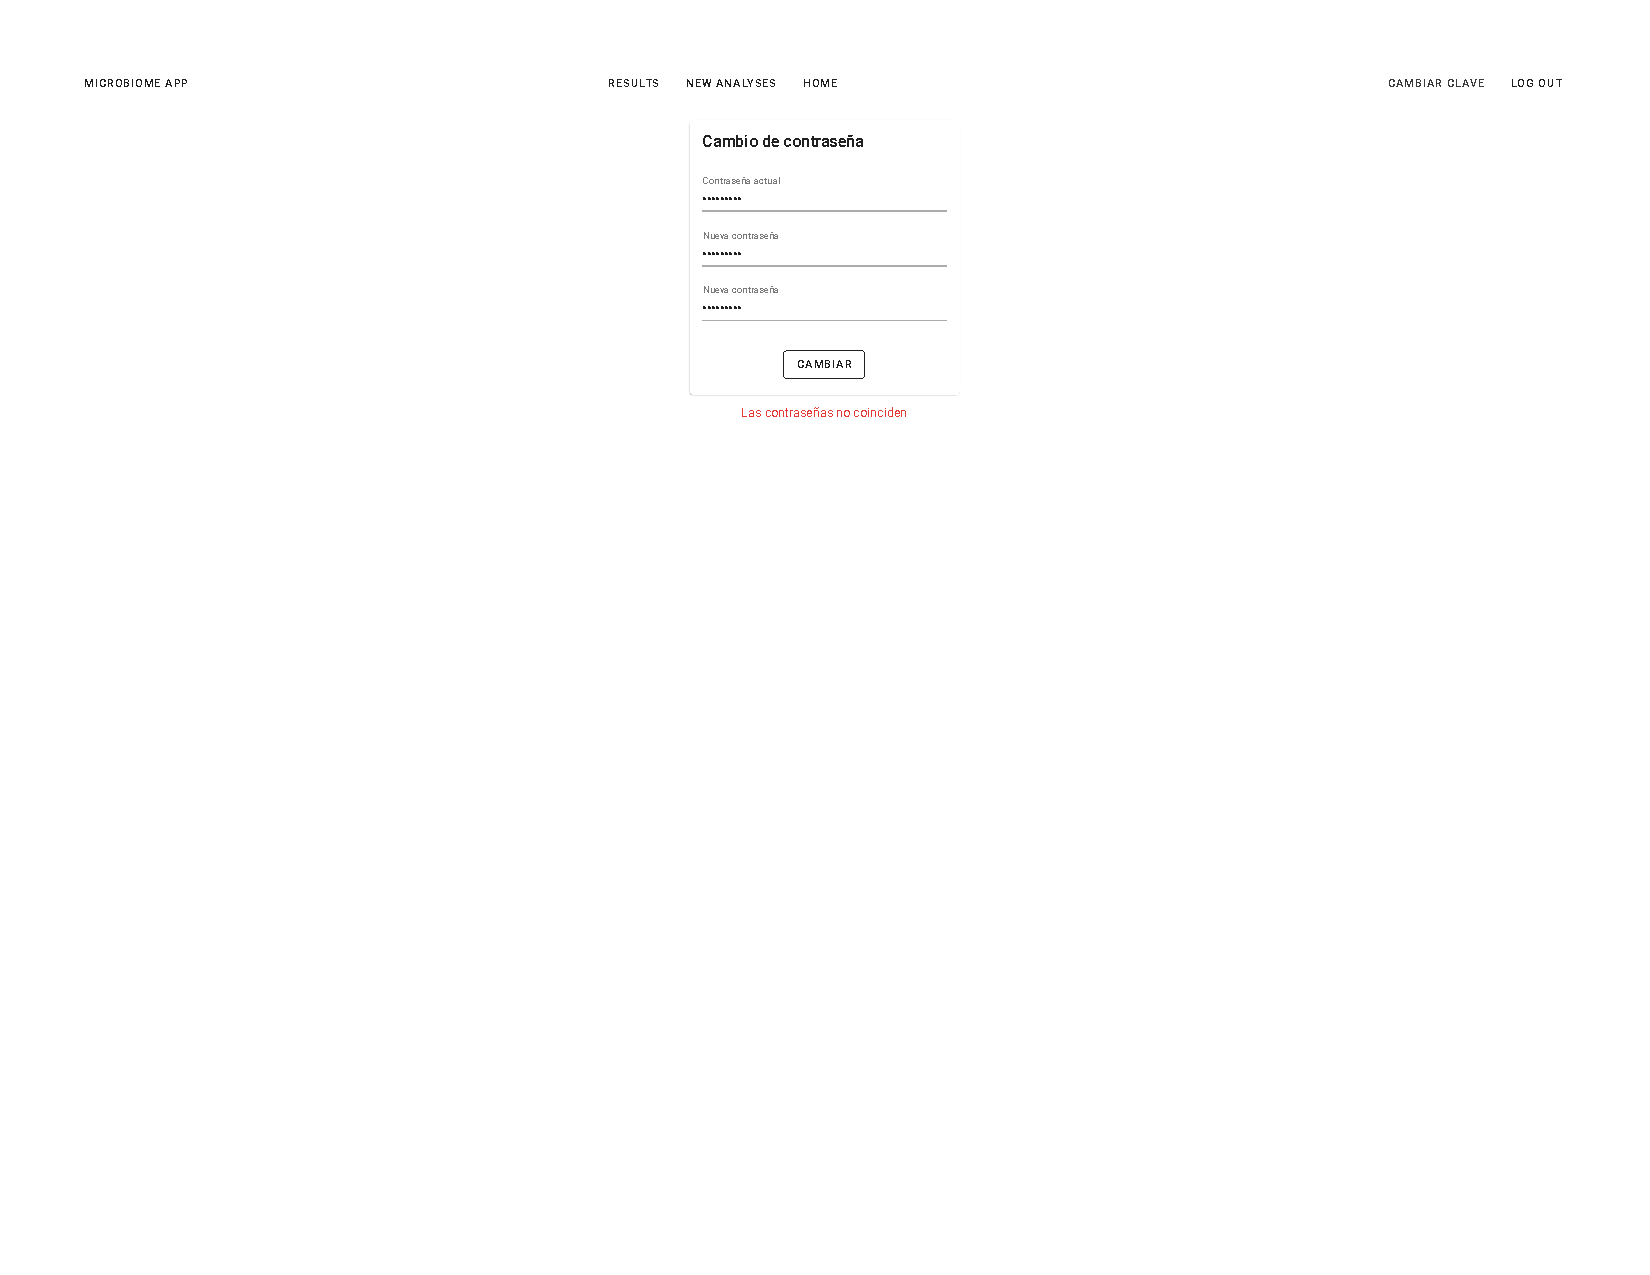
\includegraphics[width=\textwidth]{images/app/chage-psw-error2.png}
%         \caption{d}
%         \label{fig:subfig4}
%     \end{subfigure}

%     \vskip\baselineskip

%     \begin{subfigure}[b]{0.4\textwidth}
%         \centering
%         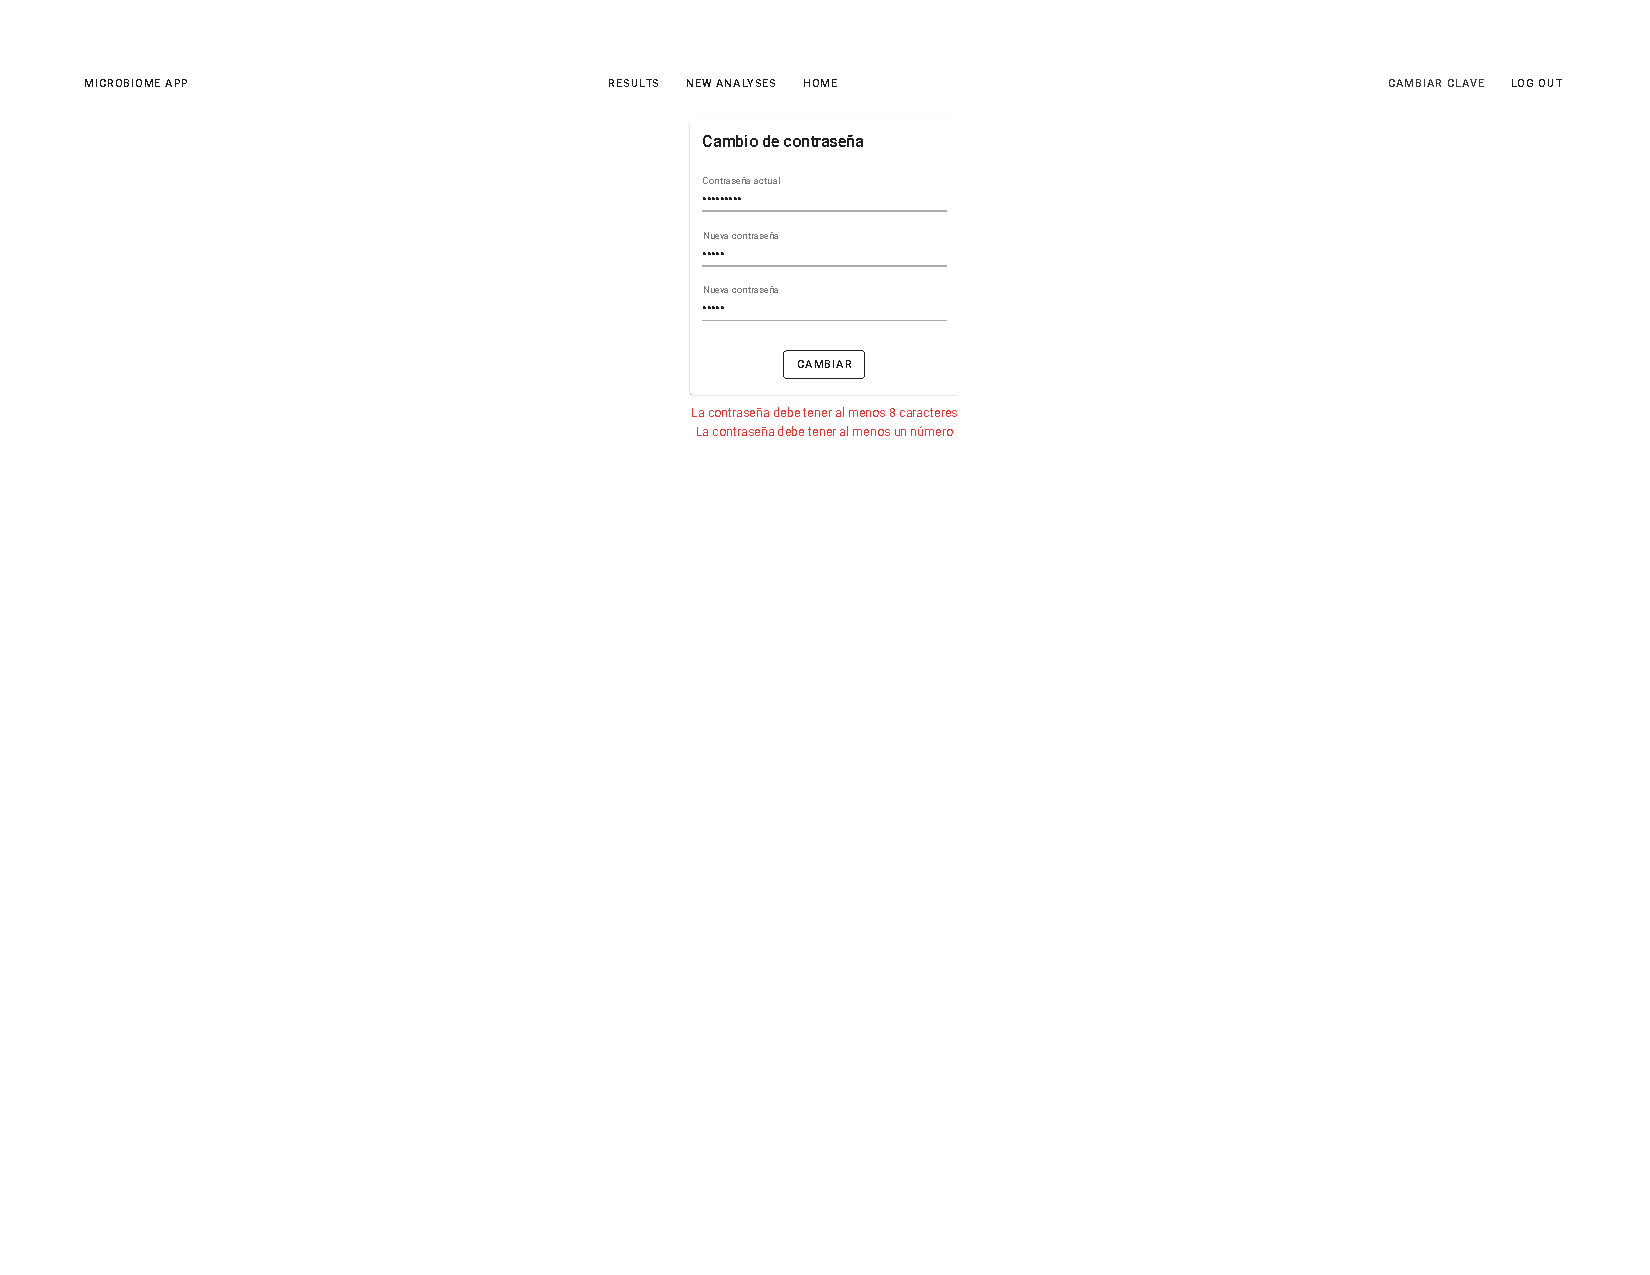
\includegraphics[width=\textwidth]{images/app/chage-psw-error3.png}
%         \caption{e}
%         \label{fig:subfig5}
%     \end{subfigure}
    
%     \caption{Título de la figura principal}
%     \label{fig:main}
% \end{figure}


\subsection{Nuevo análisis}
En esta sección el usuario deberá ingresar la información del proyecto, datos de secuenciación, y metadata para poder realizar los análisis. 
El usuario deberá rellenar la información básica del proyecto como, nombre, descripción, tipo de archivos y mediante un archivo en formato (XLXS) deberá ingresar la información de las muestras. %, como nombre de archivo, nombre de la muestra, barcode (opcional) y grupo (opcional).
Los datos de secuenciación se debe subir a algún directorio del drive del usuario y se debe dar acceso a la cuenta \textit{nanotax.catg@gmail.com}.
La figura~\ref{fig:app-new-analysis-def} presenta la vista inicial de la sección de Nuevo análisis.

\begin{figure}[H]
    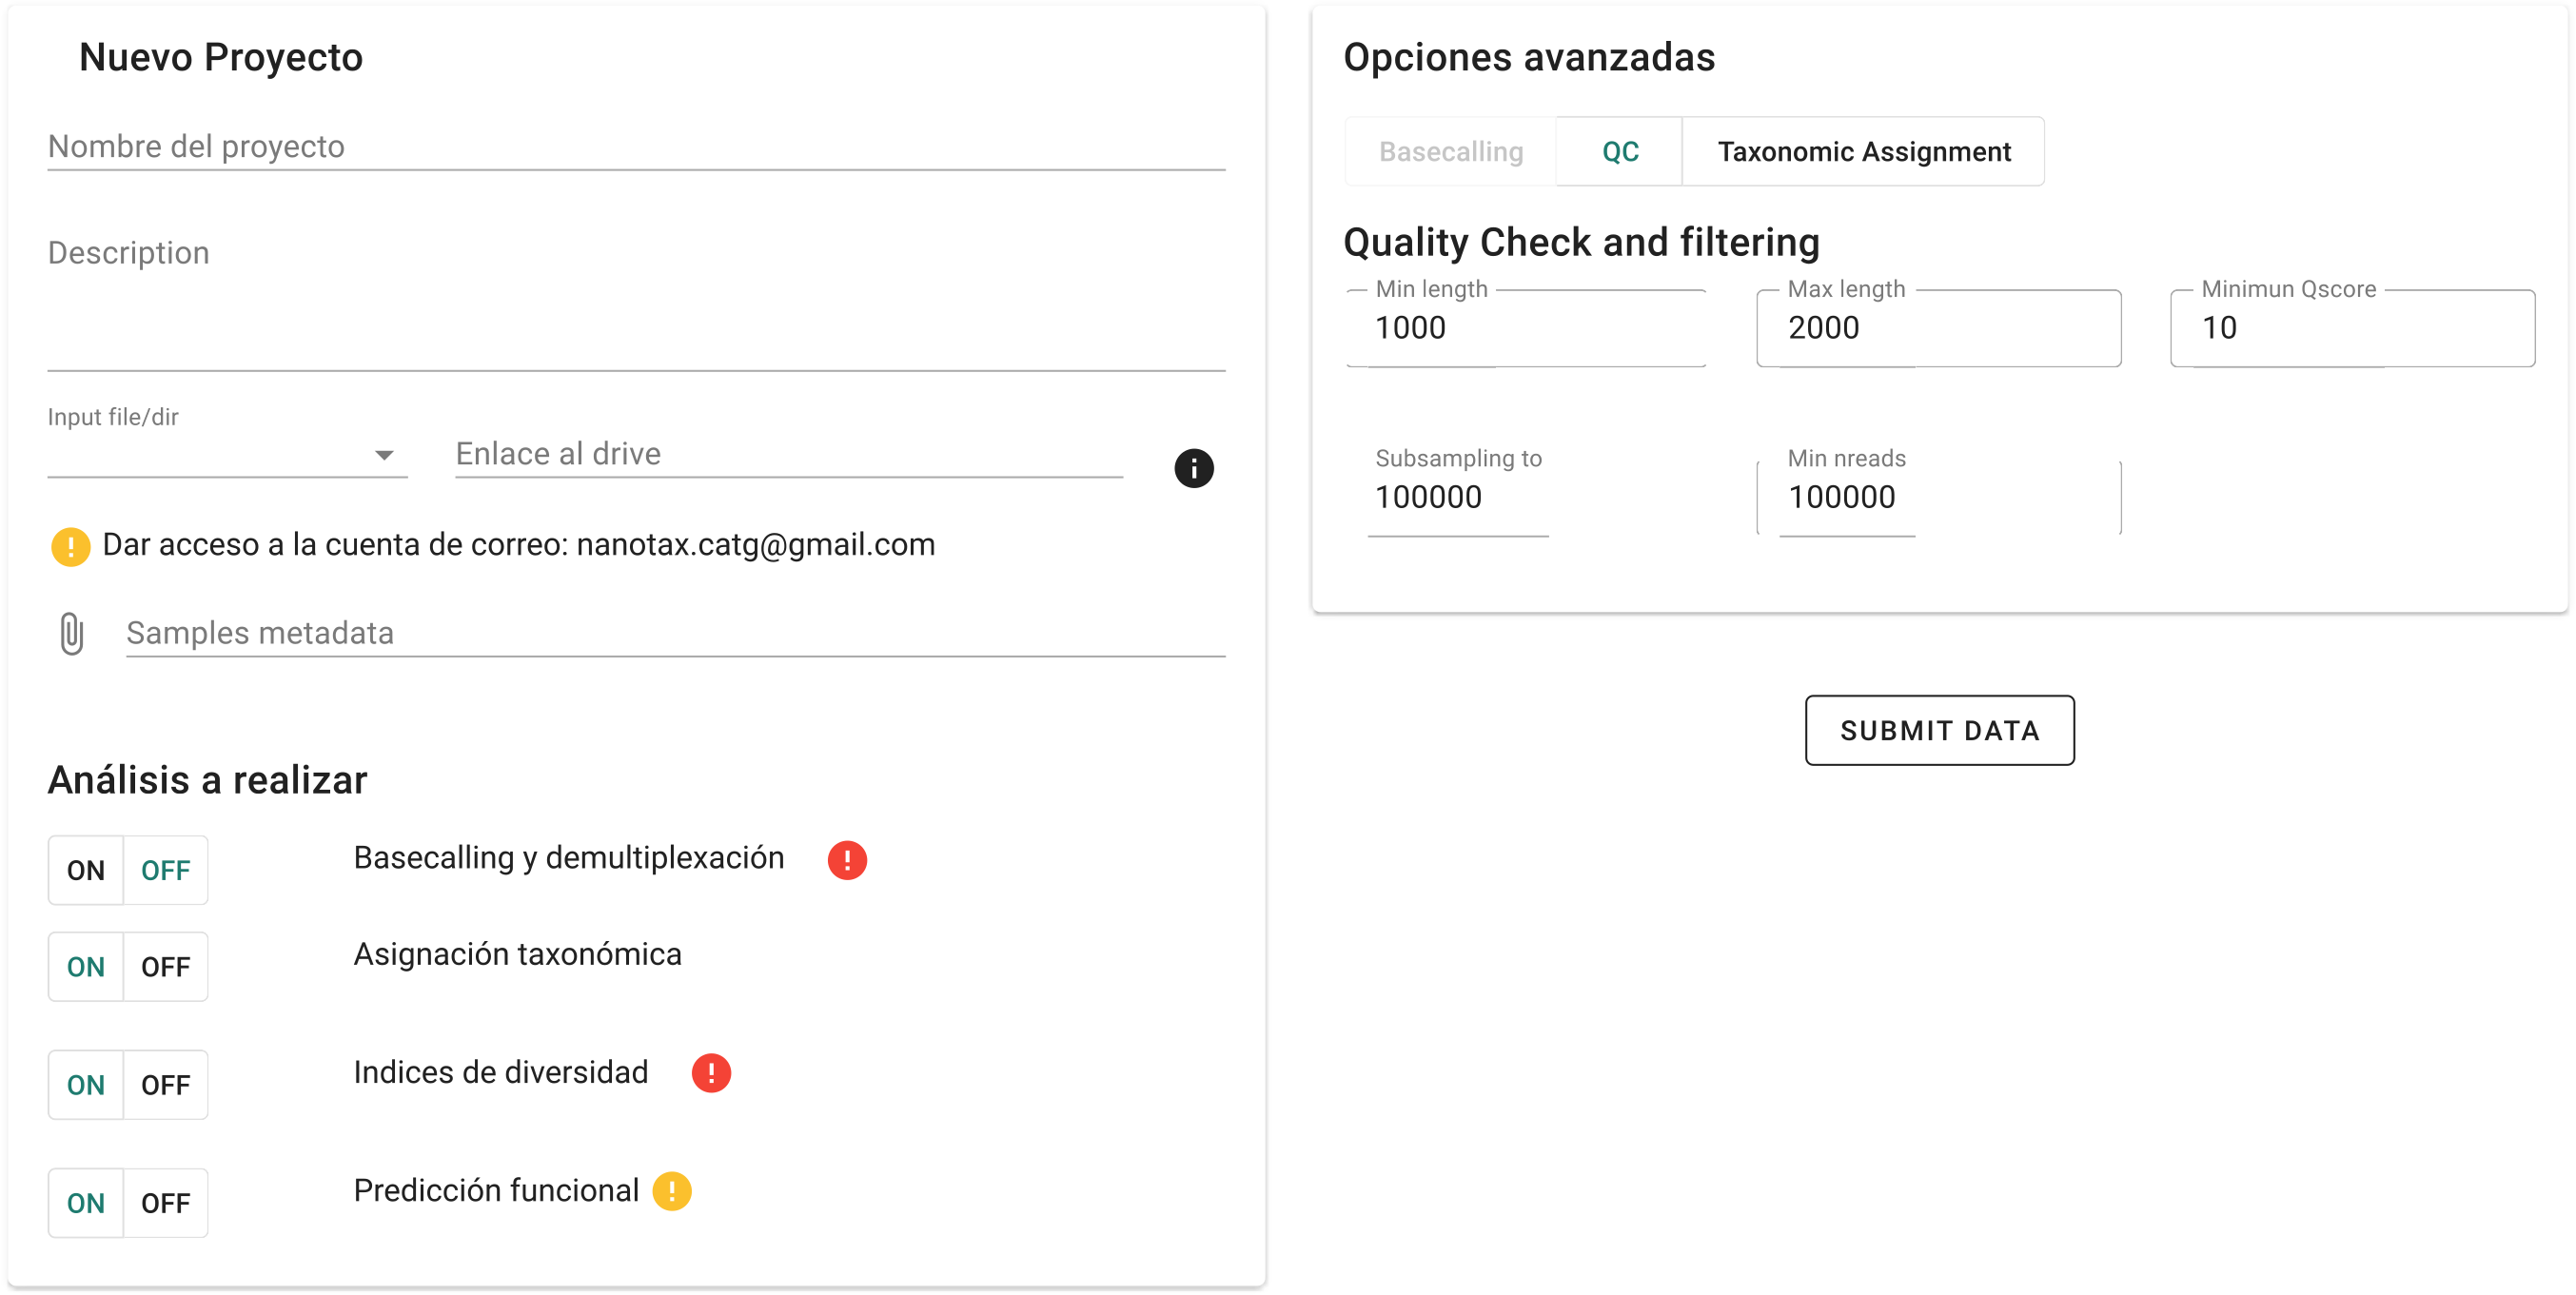
\includegraphics[width=1\linewidth]{images/app/newAnalysis/new-analysis-def.png}
    % \captionsetup{justification=raggedright, width=0.45\linewidth, singlelinecheck=off}

    % \captionsetup{width=0.45\linewidth}
    \caption{Vista por defecto de Nuevo análisis}
    \label{fig:app-new-analysis-def}
\end{figure}


A continuación se describen los datos que el usuario debe rellenar:

\begin{itemize}
    \item Nombre: Nombre del proyecto a utilizar en la plataforma (sección de visualización de proyectos y resultados).
    \item Descripción (opcional): Descripción del proyecto, campo opcional.
    \item Tipo de archivo a subir (POD5, FASTQ): Archivos de secuenciación que se procesarán:
    \begin{itemize}
        \item POD5: En caso de querer comenzar desde el proceso de basecalling y demultiplexación de las muestras.
        \item FASTQ: En caso de querer saltarse el paso de basecalling y demultiplexación e iniciar directamente con el control de calidad y asignación taxonómica.
    \end{itemize}
    \item Archivo de metadata en formato XLXS con las siguientes columnas para cada muestra:
    \begin{itemize}
        \item file: nombre del archivo subido al drive (obligatorio)
        \item sample: identificador de la muestra (obligatorio)
        \item barcode (opcional): barcode que identifica la muestra (en caso de querer realizar basecalling y demultiplexación)
        \item group (opcional): groupo al que pertenece cada muestra (en caso de querer hacer diferenciación entre grupos)
    \end{itemize}
    \item Análisis a realizar:
    \begin{itemize}
        \item Basecalling y demultiplexacion
        \item Asignación taxonomica
        \item Indices de diversidad
        \item Predicción funcional
    \end{itemize}
\end{itemize}


En el lado derecho de la vista se puede visualizar una sección de opciones avanzadas, donde el usuario puede modificar los parámetros por defecto en caso de que quiera modificar el comportamiento del pipeline (gigura~\ref{fig:app-new-analysis-def}). Esta información es seleccionados desde la base de datos la cual almacena los parámetros por defecto del flujo de trabajo.

Cabe destacar que en caso de que el directorio del drive no contenga la información necesaria, el proyecto se subirá correctamente y luego pasara a un estado de datos inválidos.
Los filtros y control de calidad se realizan siempre por lo que no aparecerá la opción en la lista de análisis.
Por defecto basecalling y demuliplexación se encuentra deshabilitado, en caso de que el usuario desee realizar este análisis deberá seleccionarlo, y al hacerlo se desbloqueará la sección de configuración de este análisis (Figura~\ref{fig:app-new-analysis-basecallingON}).



\begin{figure}[H]
    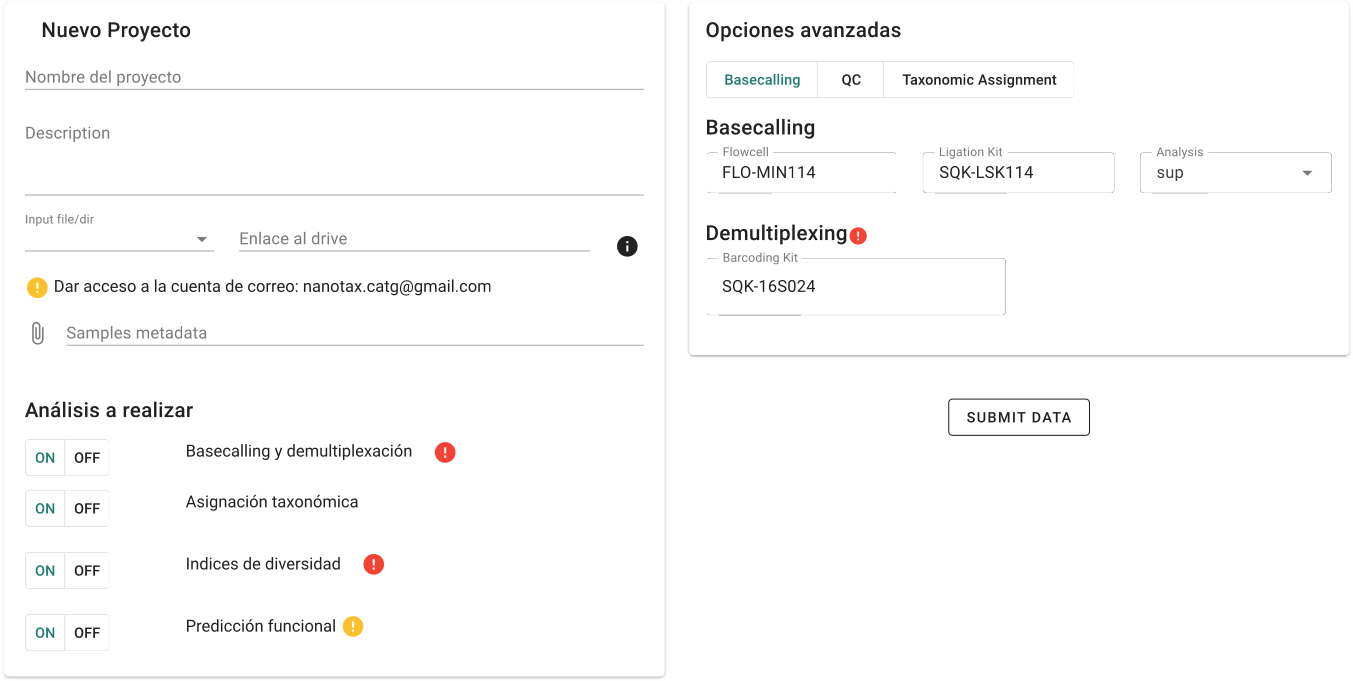
\includegraphics[width=1\linewidth]{images/app/newAnalysis/new-analysis-basecallingON.png}
    % \captionsetup{justification=raggedright, width=0.45\linewidth, singlelinecheck=off}

    % \captionsetup{width=0.45\linewidth}
    \caption{Vista de Nuevo análisis habilitando la opción de basecalling y demultiplexación}
    \label{fig:app-new-analysis-basecallingON}
\end{figure}
% La plataforma se encarga de verificar si el archivo de metadata cuenta con la información necesaria para realizar cada analisis. En caso de que el archivo de metadata no cuente con la información necesaria y el usuario desee realizar uno de esos analisis, se desplegara un mensaje de error al lado del análisis indicando que información se debe añadir en el archivo de metadata. Los parámetros que se pueden modificar son los siguientes:
% \begin{itemize}
%     \item Basecalling y demultiplexacion: Flowcell, kit de ligación y kit de barcoding utilizados durante la secuenciación. Modelo a utilizar para realizar el basecalling
%     \item QC: Longitud mínima y máxima en pares de bases de las lecturas, calidad mínima de las lecturas y cantidad de lecturas a utilizar para los análisis posteriores(subsampleo).
%     \item Predicción funcional: \hl{completar}
% \end{itemize}

% En la parte derecha del componente el usuario puede visualizar los parámetros por defecto y modificarlos en caso de que lo desee. 


Una vez que el usuario presione al botón \textit{Subir proyecto}, la plataforma realiza un proceso de validación para verificar que toda la información subida por el usuario sea correcta. En caso de no serla, la plataforma no permitirá subir el proyecto y podrá presentar alguno de los siguientes mensajes de error:
\begin{itemize}
    \item En caso de no completar el nombre del proyecto o el enlace al directorio del drive ambos campos pasarán a estar en color rojo (figura ~\ref{fig:app-new-analysis-type-file-error}).
    \item En caso de no seleccionar el tipo de archivo a subir, este campo pasará a estar en color rojo y se presentará el siguiente mensaje: \textit{Debe seleccionar el formato de los archivos de entrada} (figura ~\ref{fig:app-new-analysis-type-file-error}).
    \item En caso de seleccionar el formato de archivo \textit{POD5} y no haber seleccionado el proceso de basecalling y demultiplexación como inicio se presentará el mensaje: \textit{Al iniciar con basecalling debe subir los archivos POD5} (figura ~\ref{fig:app-new-analysis-type-file-error}).
    \item En caso de seleccionar el formato de archivo \textit{FASTQ} y haber seleccionado el proceso de basecalling y demultiplexación como inicio se presentará el mensaje: \textit{Al iniciar con QC o asignación taxonómica debe subir los archivos FASTQ} (figura ~\ref{fig:app-new-analysis-type-file-error}).
    \item En caso de que el archivo de metadata no cuente con todas las columnas necesarias se pueden presentar uno o más de los siguientes mensajes de errores (figura ~\ref{fig:app-new-analysis-type-file-error}):
    \begin{itemize}
        \item \textit{El archivo de metadata le falta la columna file}
        \item \textit{El archivo de metadata le falta la columna sample}
        \item \textit{El archivo de metadata le falta la columna barcode}: Solo en caso de seleccionar basecalling y demultiplexación como inicio del pipeline.
        \item \textit{El archivo de metadata le falta la columna group}: Solo en caso de querer realizar análisis por grupos (índices de diversidad).

    \end{itemize}
\end{itemize}


\begin{figure}[H]
    \centering
    \begin{subfigure}[b]{0.45\textwidth}
        \centering
        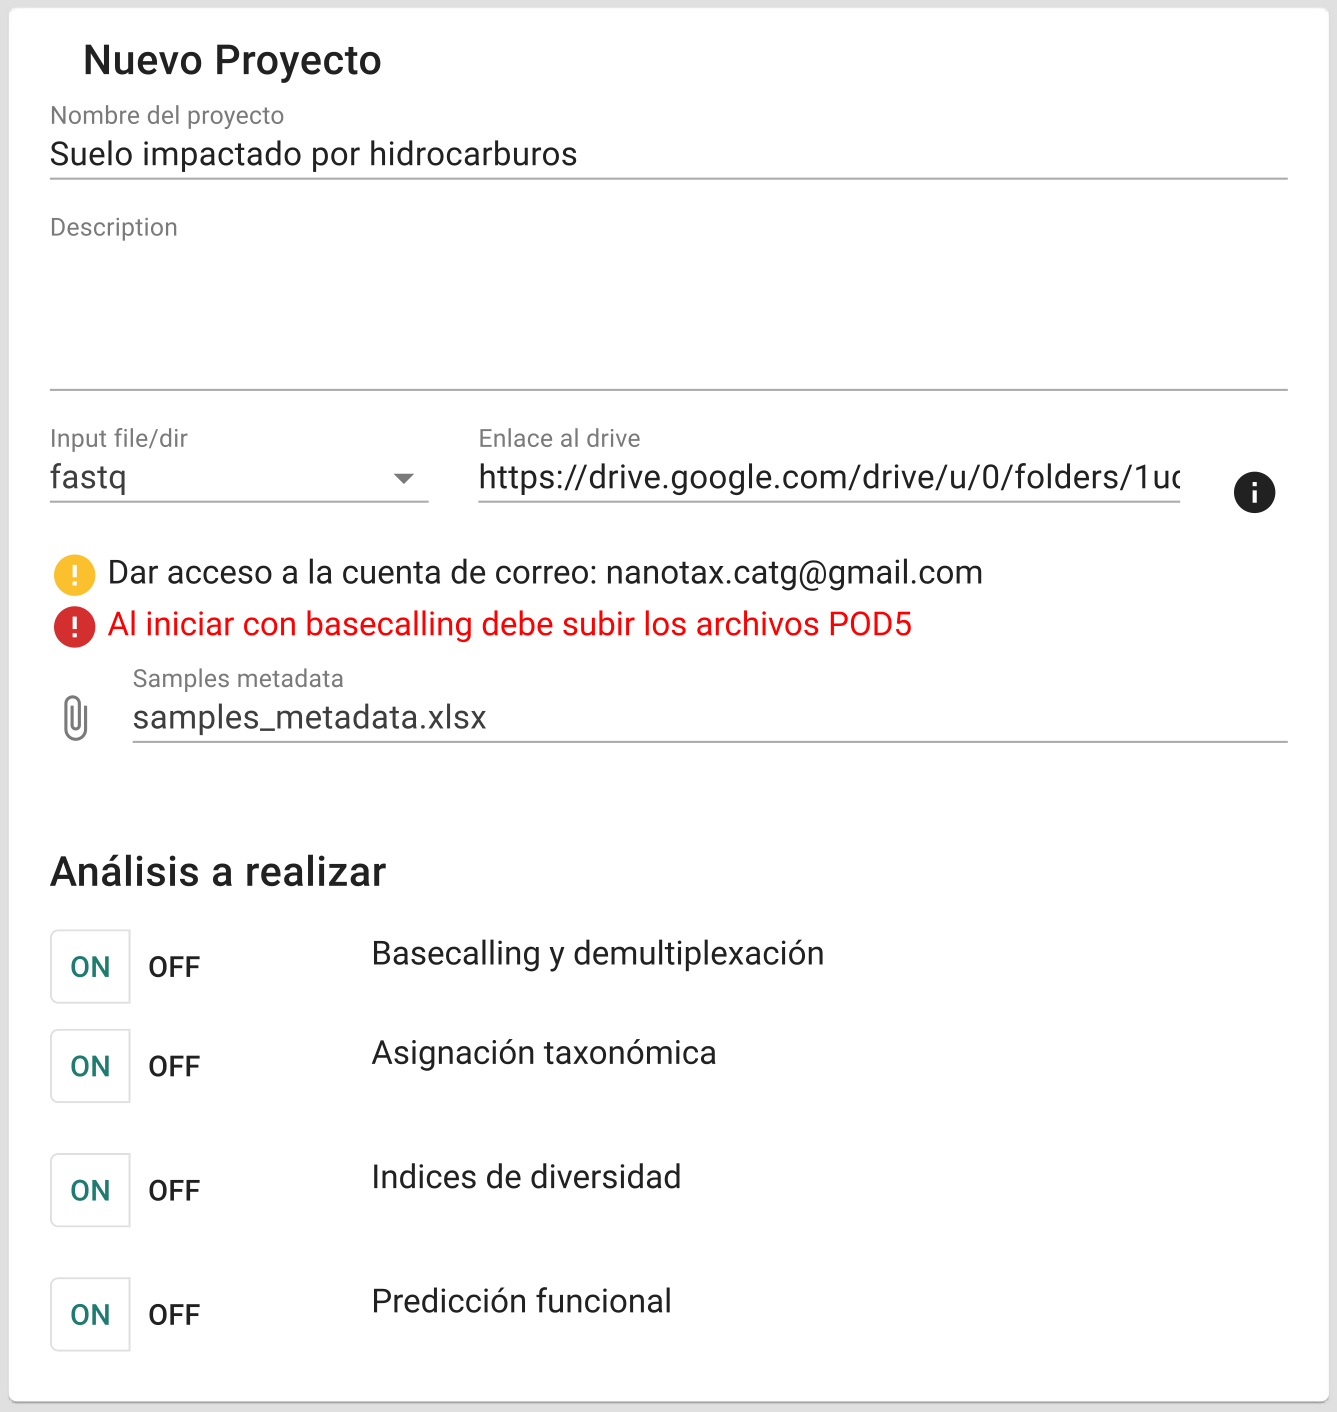
\includegraphics[width=\textwidth]{images/app/newAnalysis/pod5-error.png}
        \caption{Vista de nuevo análisis: Error al seleccionar el tipo del archivo}
        \label{fig:app-new-analysis-pod5-error}
    \end{subfigure}
    \hfill
    \begin{subfigure}[b]{0.45\textwidth}
        \centering
        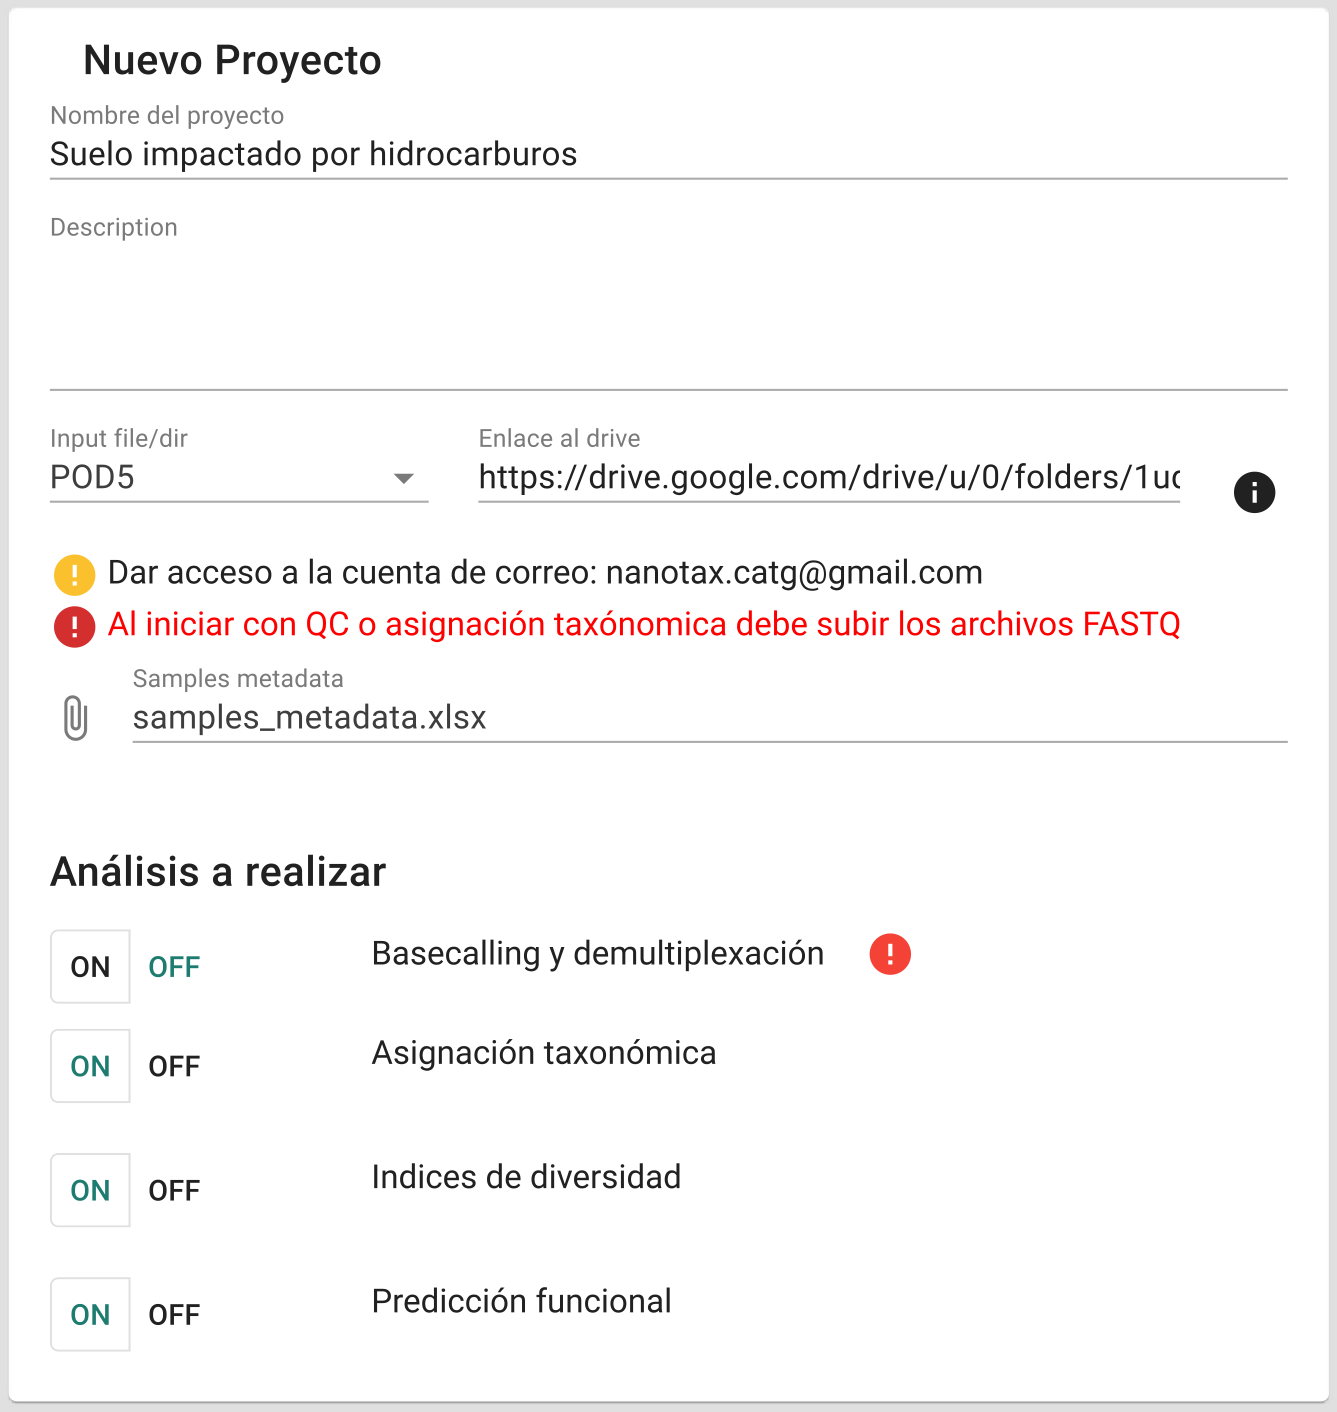
\includegraphics[width=\textwidth]{images/app/newAnalysis/fastq.png}
        \caption{Vista de nuevo análisis: Error al seleccionar el tipo del archivo}
        \label{fig:app-new-analysis-fastq-error}
    \end{subfigure}
    \caption{Vista de nuevo análisis: Error al seleccionar el tipo del archivo}
    \label{fig:app-new-analysis-type-file-error}
\end{figure}



\begin{figure}[H]
    \centering
    \begin{subfigure}[b]{0.45\textwidth}
        \centering
        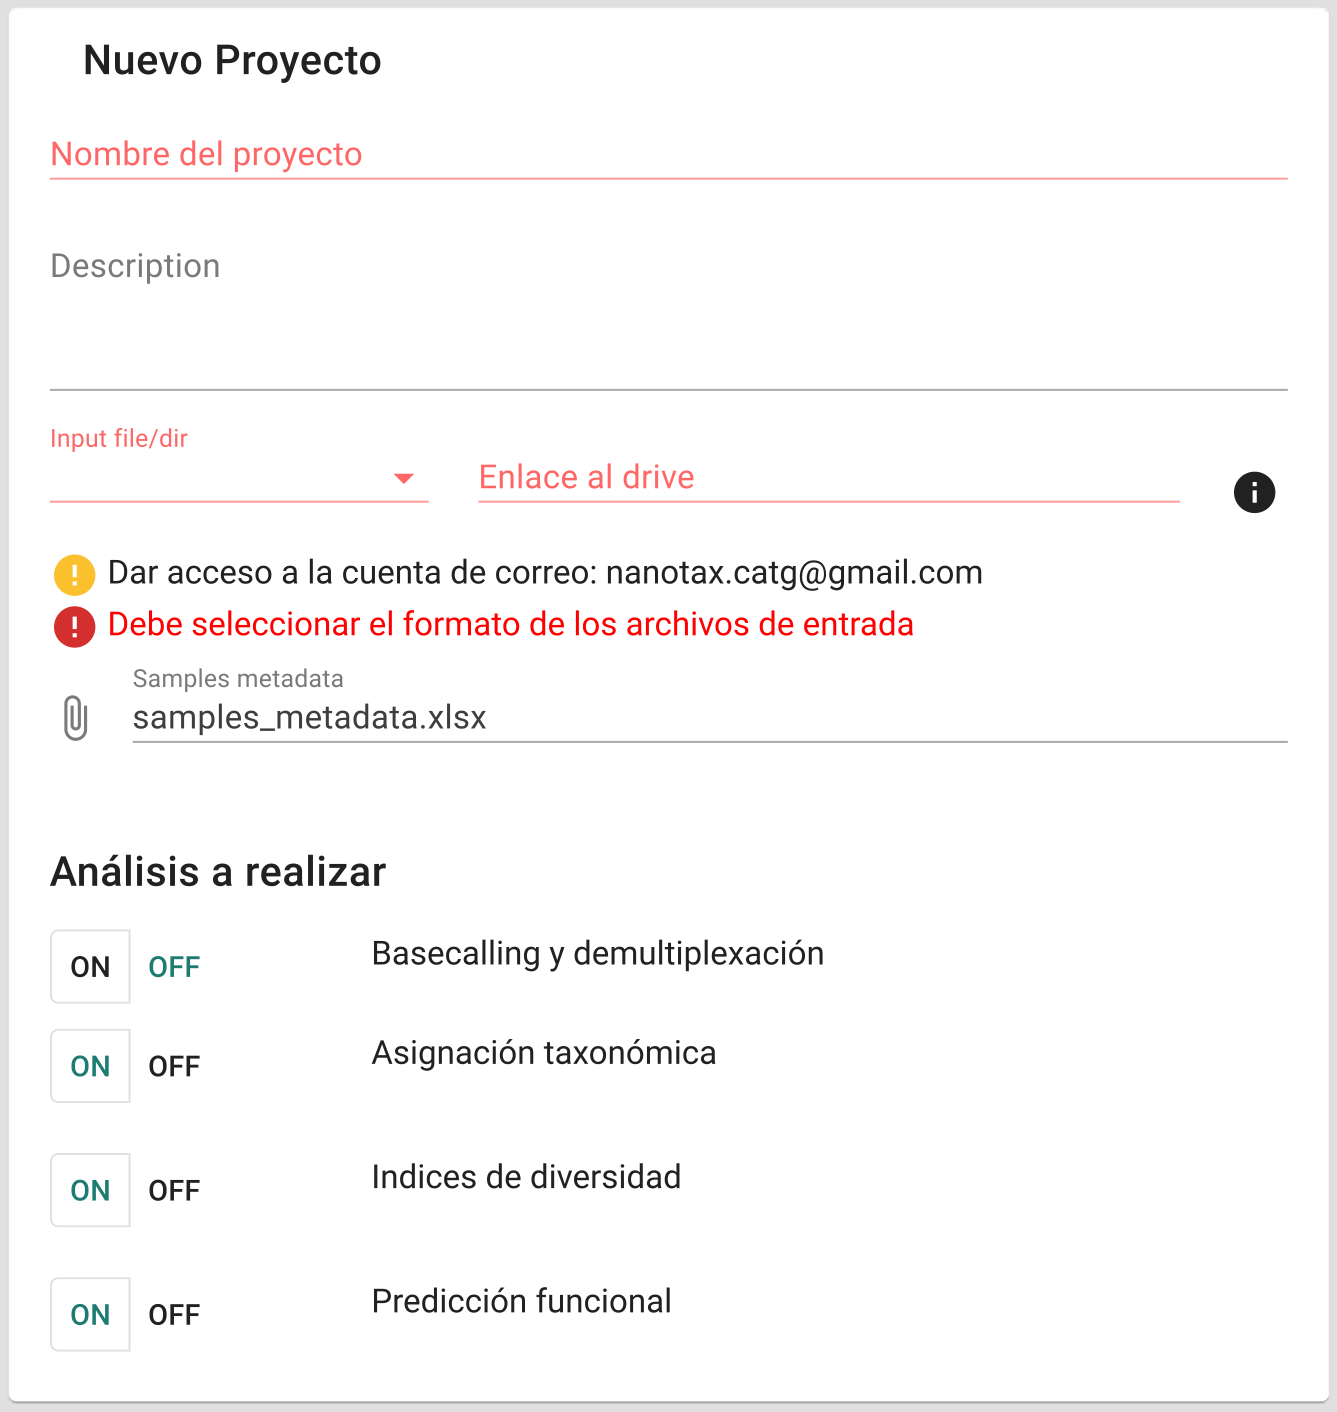
\includegraphics[width=\textwidth]{images/app/newAnalysis/errors1.png}
        \caption{Vista de nuevo análisis: Errores por falta de información}
        \label{fig:app-new-analysis-nodata-error}
    \end{subfigure}
    \hfill
    \begin{subfigure}[b]{0.45\textwidth}
        \centering
        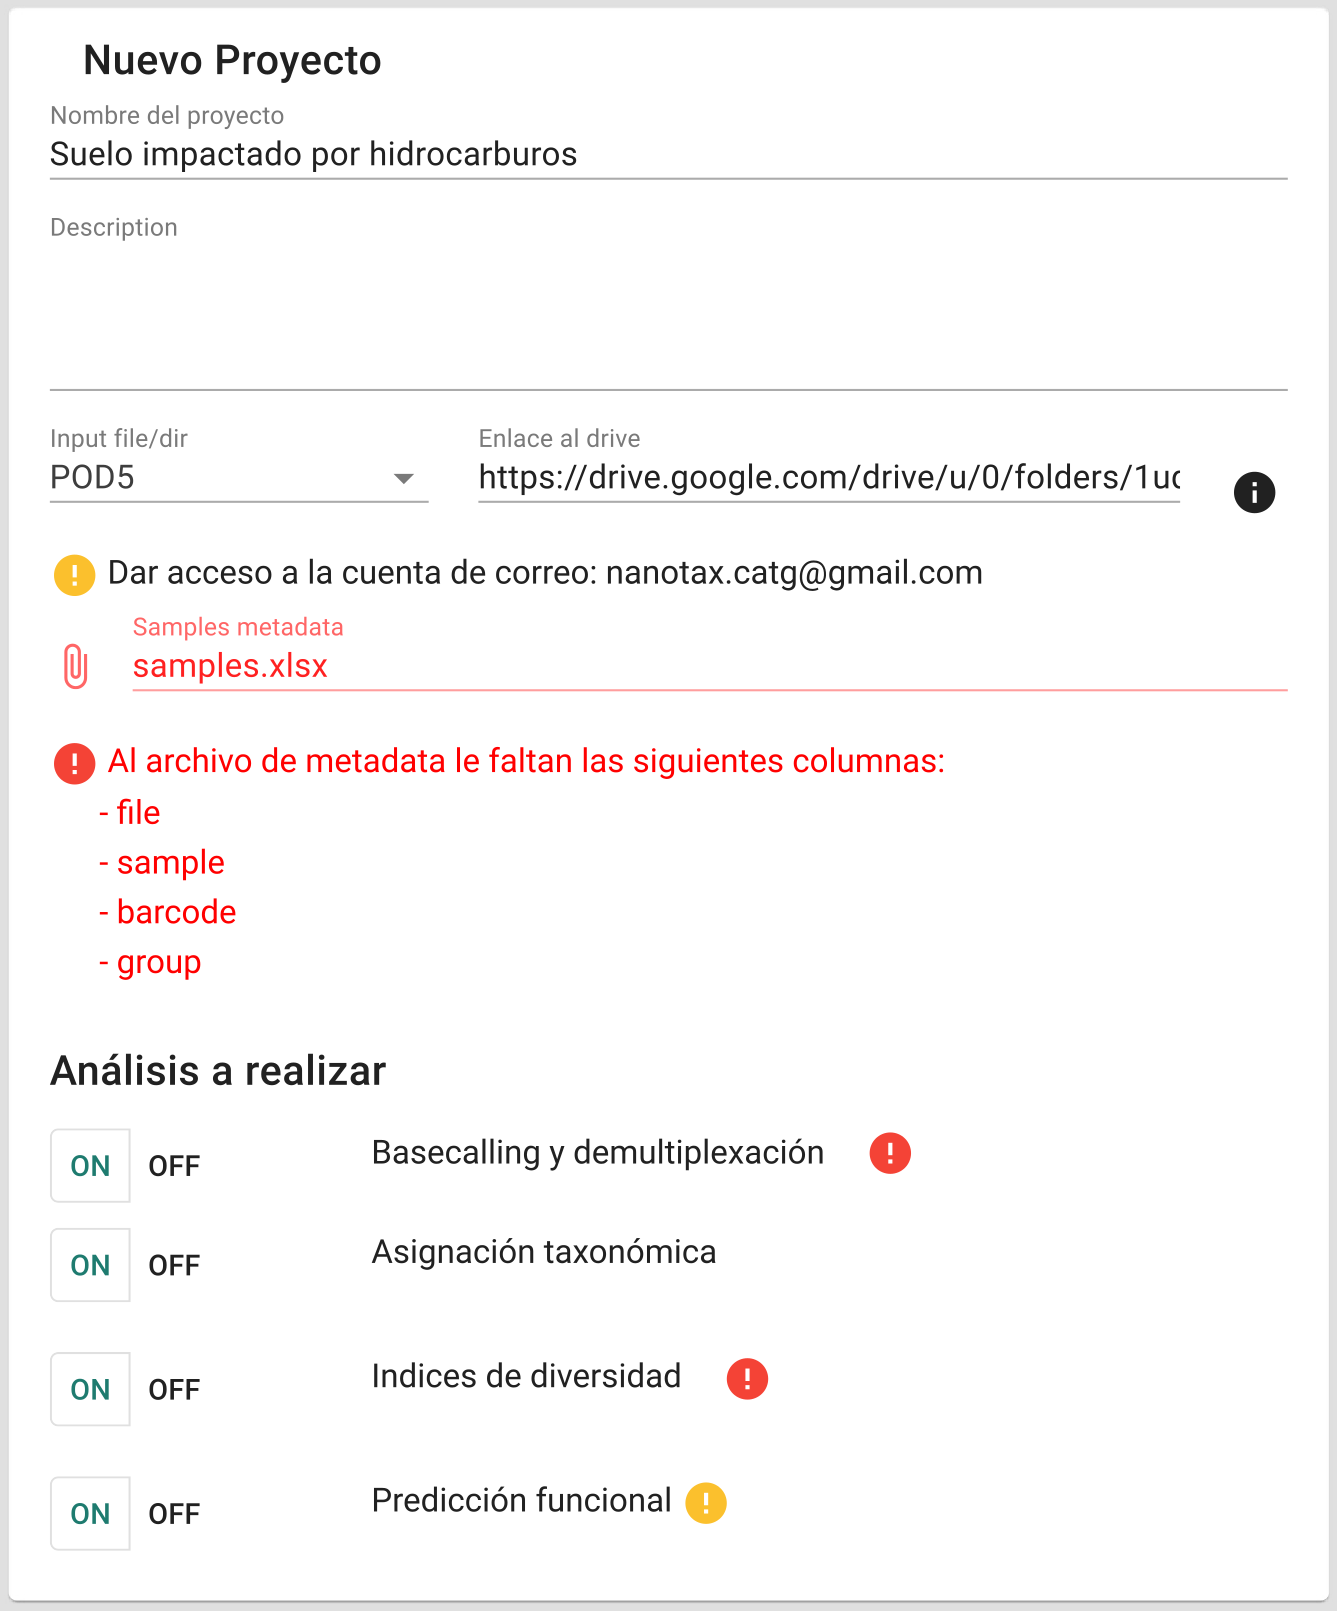
\includegraphics[width=\textwidth]{images/app/newAnalysis/metadata-error-1.png}
        \caption{Vista de nuevo análisis: Errores en el archivo de metadata}
        \label{fig:app-new-analysis-metadata-error}
    \end{subfigure}
    \caption{Vista de nuevo análisis: Errores }
    \label{fig:app-new-analysis-metadata-nodata-error}
\end{figure}



En la parte inferior del componente se encuentra el botón de Subir data, el cual al hacer click en el, ingresará la información a la base de datos y copiará los archivos a la plataforma de computo. Una vez que el usuario presionar el botón de subir data, la plataforma se encarga de verificar que se cuente con toda la información necesaria para correr el pipeline.





%%%%%%%%%%%%%%%%%%%%%%%%%%%%%%%%%%%%%%%%%%%%%%%%%%%%%%%%%%%%%%%%%%%%%%

\subsection{Resultados/Proyectos} \label{projects}
Una vez que el usuario valida sus credenciales en la plataforma será redireccionado a la sección de Resultados. En esta sección se mostraran los proyectos que el usuario ha subido a la plataforma, estos proyectos pueden estar en ejecución, finalizados o finalizados con errores. 
Por cada proyecto se desplegará la información básica en una tarjeta:
\begin{itemize}
    \item Nombre del proyecto
    \item Descripción del proyecto
    \item Cantidad de muestras procesadas, descartadas y totales
    \item Estado del proyecto (corriendo, finalizado, subido con errores)
    \item En caso de que el proyecto haya finalizado el usuario podrá acceder a la sección especifica de resultados del proyecto mediante el botón de Ver resultados.
\end{itemize}

A continuación se presenta un ejemplo de la vista de proyectos subidos a la plataforma (Figura~\ref{fig:app-results-projects}).
El primer proyecto se encuentra \textit{corriendo} por lo que no se tiene acceso a los resultados (botón de de ver resultados) ni a la información de las muestras descartadas ni analizadas correctamente.
El segundo proyecto se encuentra finalizado, por lo que se puede acceder a los resultados y se puede visualizar además la cantidad de muestras procesadas, descartadas y totales. 

\begin{figure}[H]
    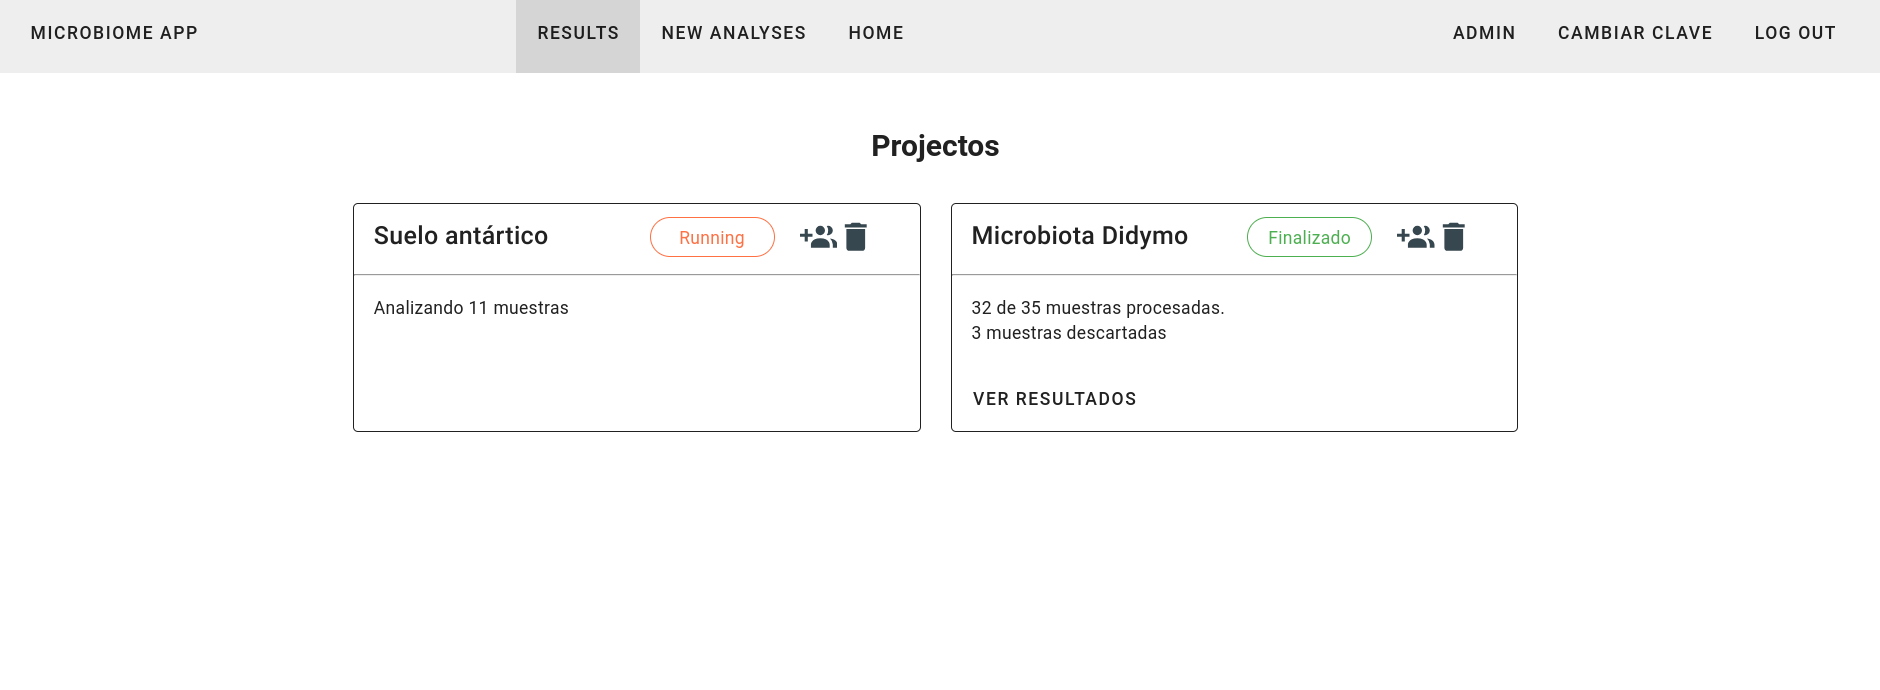
\includegraphics[width=1\linewidth]{images/app/projects.png}
    % \captionsetup{justification=raggedright, width=0.45\linewidth, singlelinecheck=off}

    % \captionsetup{width=0.45\linewidth}
    \caption{Vista de proyectos subidos a la plataforma}
    \label{fig:app-results-projects}
\end{figure}
En la parte superior de la tarjeta del proyecto se pueden visualizar dos íconos, uno para eliminar el proyecto y otro para poder compartir los resultados del proyecto con otros usuarios de la plataforma.


En el caso de seleccionar el botón para añadir usuarios se desplegará una ventana emergente donde se podrá ingresar el nombre de usuario al que se desea compartir los resultados del proyecto(Figura~\ref{fig:app-add-project}). 
En caso de que el usuario no exista en la plataforma se mostrará un mensaje de error \textit{“Usuario no encontrado”} (Figura~\ref{fig:app-add-project-invalid-usar}).
\begin{figure}[H]
        \centering
        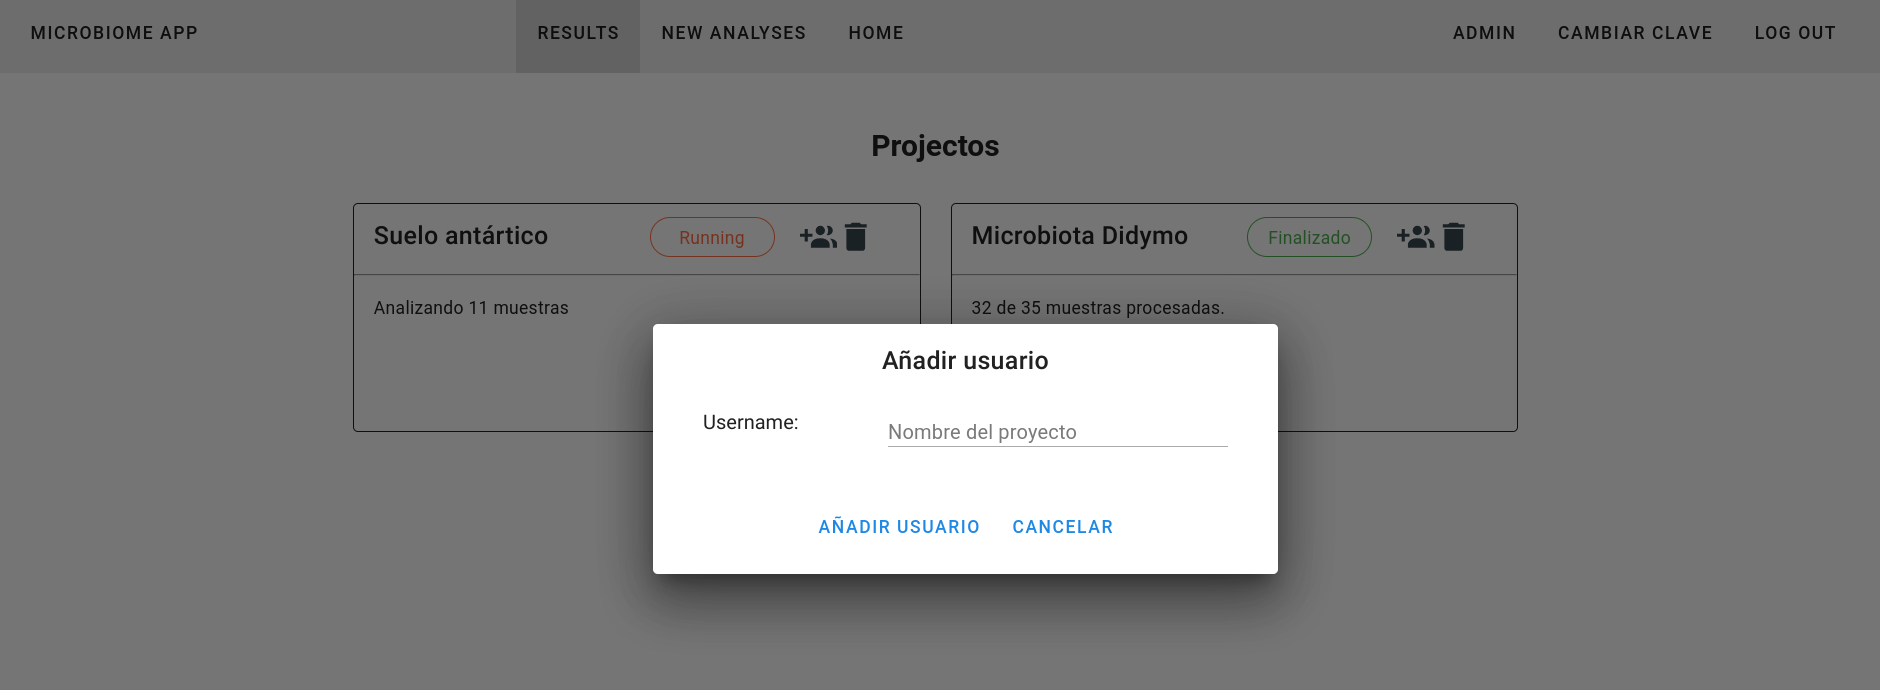
\includegraphics[width=\textwidth]{images/app/addUser.png}
        \caption{Añadir usuario a un proyecto existente}
        \label{fig:app-add-project}

\end{figure}

\begin{figure}[H]
    \centering
    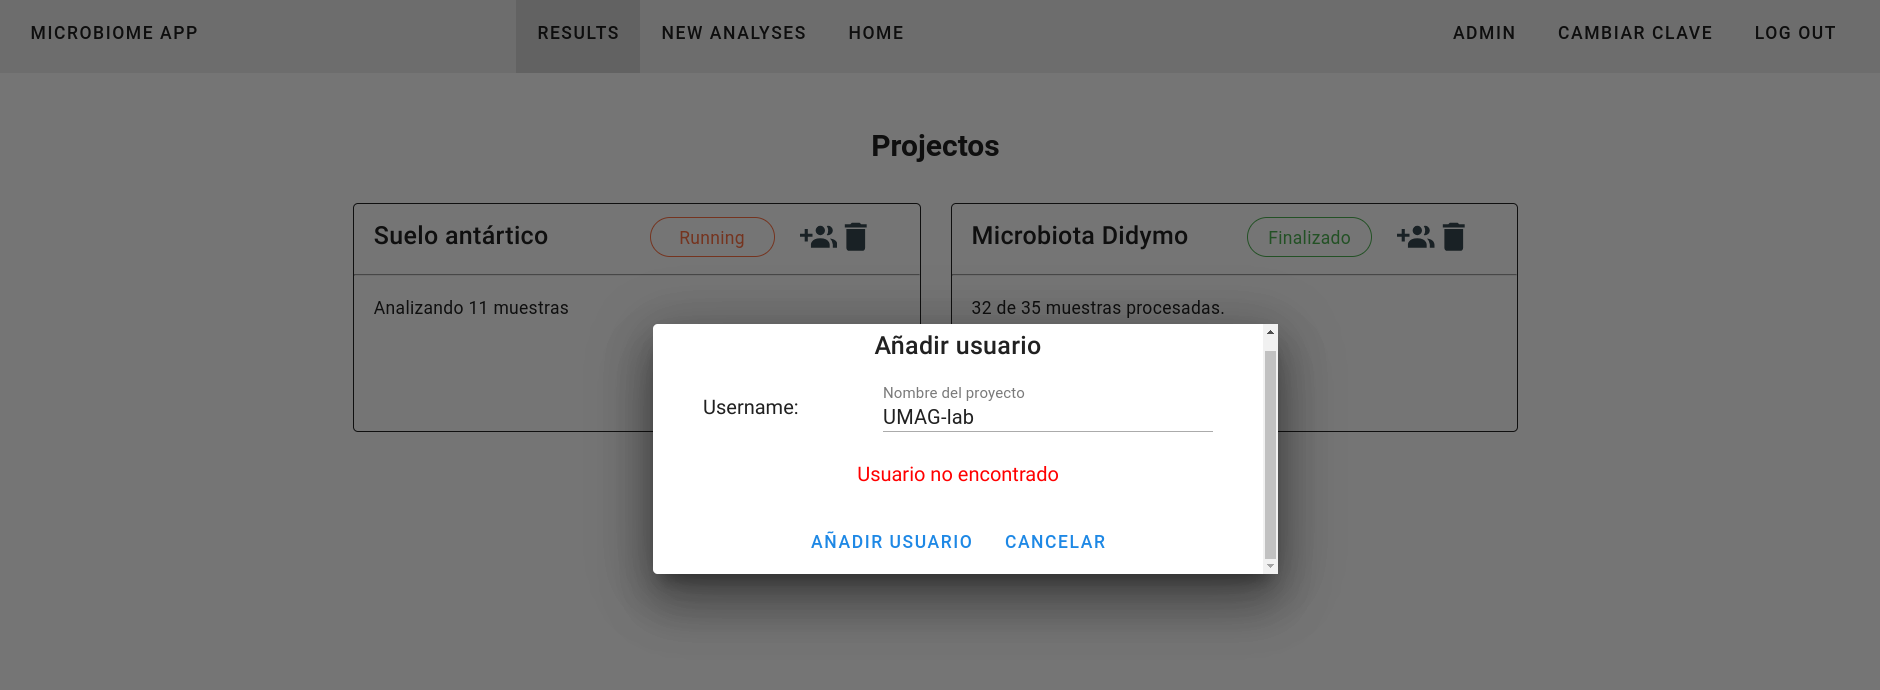
\includegraphics[width=\textwidth]{images/app/addUser_notFound.png}
    \caption{Añadir usuario a un proyecto existente: Mensaje de error debido a que el usuario no existe en la plataforma}
    \label{fig:app-add-project-invalid-usar}

\end{figure}

En el caso de seleccionar el icono para eliminar el proyecto se desplegará una ventana emergente con un mensaje de confirmación, en caso de confirmar la eliminación del proyecto se eliminará toda la información asociada al proyecto de la base de datos y se eliminarán los archivos asociados al proyecto de la plataforma de computo~\ref{fig:app-delete-project}.

\begin{figure}[H]
    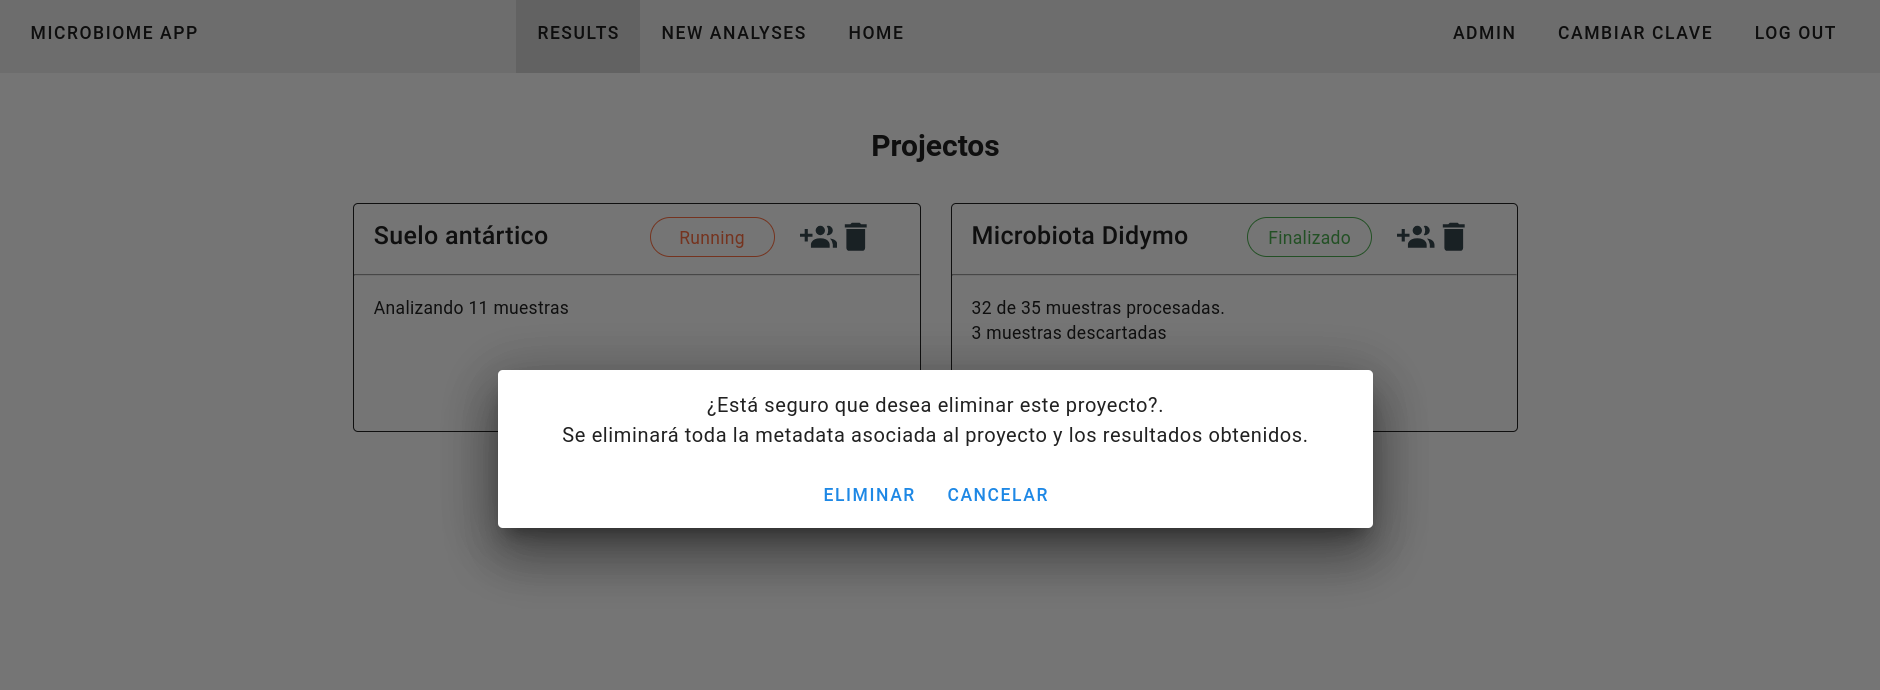
\includegraphics[width=1\linewidth]{images/app/deleteProject.png}
    % \captionsetup{justification=raggedright, width=0.45\linewidth, singlelinecheck=off}

    % \captionsetup{width=0.45\linewidth}
    \caption{Eliminar proyecto de la plataforma}
    \label{fig:app-delete-project}
\end{figure}

\subsection{Resultados de un proyecto en especifico}
Una vez que el pipeline haya finalizado su ejecución, la plataforma permitirá al usuario acceder a los resultados de cada proyecto leyendo los resultados desde la base de datos y desplegando la información en la sección de resultados de cada proyecto.
Esta sección cuenta con 5 subsecciones, cada una con información específica del análisis realizado. 
En caso de que al ingresar el proyecto el usuario no seleccione todos los análisis, solo se mostrarán las secciones indicadas por el usuario.

\subsection{Información básica de las muestras}
%Esta sección se mostrará siempre que el usuario empiece con archivos POD5 o FastQ, es decir, ya sea comenzando el análisis desde el basecalling o desde el control de calidad. \hl{Igual si es que solo se hace asignaicón taxonomica}.
Esta sección se desplegará siempre en la plataforma y cuenta en el lado izquierdo con una tabla con información básica de las muestras y en el lado derecho un gráfico que representa la calidad y tamaño promedio de las lecturas.
La tabla esta compuesta por los siguientes elementos:
\begin{itemize}
    \item Nombre de la muestra: Nombre indicado en el archivo de metadata al ingresar el proyecto.
    % \item \hl{Grupo}: Grupo asociado a la muestra en el archivo de metadata (en caso de ingresar grupo).
    \item Total de lecturas: Cantidad de lecturas previo a los filtros de calidad.
    \item Calidad promedio: Calidad promedio en formato phred despues de los filtros de calidad.
    \item Largo promedio: Largo promdio despues de los filtros de calidad
    \item Lecturas después de los filtros: Cantidad de lecturas luego de los filtros de calidad.
    \item Nota: Si la muestra fue descartada por no contar con la cantidad suficiente de lecturas se informará en esta columna.
\end{itemize}
En la parte inferior de la tabla hay una nota que indica la cantidad de lecturas que se consideraron para los análisis posteriores, este valor por defecto es 100.000, pudiendo ser modificado por el usuario en las opciones avanzadas al ingresar el proyecto.

En la parte derecha de la sección se puede visualizar un heatmap donde en el eje X se encuentra el tamaño de las secuencias, y en el eje Y la calidad. 
El color indica la cantidad de lecturas que se encuentran en esa intersección, mientras más intenso el color, más secuencias tienen la calidad y tamaño indicado.
Para este grafico se consideraron todas las muestras con sus lecturas después de los filtros de calidad.

% En la parte inferior del gráfico hay una nota que indica en que rangos de tamaño se encuentran la mayoria de las lecturas\hl{Muy generico?}. 
A continuación se presenta un ejemplo de la sección de información básica de las muestras (Figura~\ref{fig:app-results-basicStatistics}).
\begin{figure}[H]
    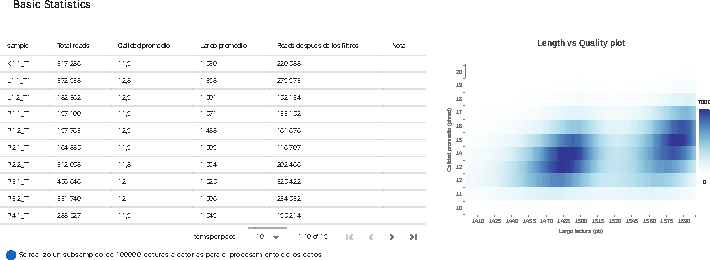
\includegraphics[width=1\linewidth]{images/app/results/basicStatistics.pdf}
    % \captionsetup{justification=raggedright, width=0.45\linewidth, singlelinecheck=off}

    % \captionsetup{width=0.45\linewidth}
    \caption{Estadisticas básicas (resultados)}
    \label{fig:app-results-basicStatistics}
\end{figure}

En caso de que el usuario ingrese un valor mínimo de lecturas para realizar los análisis y alguna de las muestras no cumpla con este valor, se mostrará un mensaje de error en la tabla de información básica de las muestras (Figura~\ref{fig:app-results-basicStatistics-exclude}).
\begin{figure}[H]
    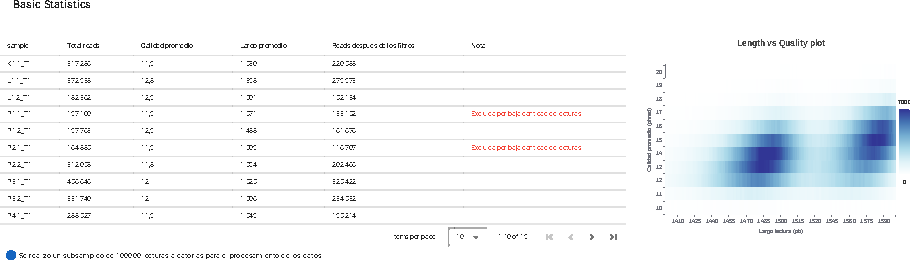
\includegraphics[width=1\linewidth]{images/app/results/basicStatistics_exclude.pdf}
    % \captionsetup{justification=raggedright, width=0.45\linewidth, singlelinecheck=off}

    % \captionsetup{width=0.45\linewidth}
    \caption{Estadisticas básicas (resultados)}
    \label{fig:app-results-basicStatistics-exclude}
\end{figure}

\subsection{Asignación taxonómica}
En la parte superior de esta sección se pueden visualizar pestañas que representan cada categoría taxonómica (especie, género, familia, orden, clase y filo), las cuales permiten ajustar la visualización de la información presentada en esta  sección (gráfico de barras apiladas y tabla). Por defecto se presenta la información para la categoría de especie.

Debajo de las pestañas en el lado izquierdo hay un gráfico de barras apiladas que permite visualizar la abundancia de las taxonomías en cada muestra.
El usuario puede interactuar con el gráfico modificando la visualización a través de los botones que se encuentran en la parte inferior, pudiendo visualizar la información en porcentaje o en cantidad de lecturas, como también pudiendo modificar el porcentaje mínimo para crear la categoria \textit{Otros}.
En caso de que el usuario hubiera ingresado información de grupos asociados a las muestras, se podrá visualizar un nuevo grupo de botones que permite al usuario visualizar la información de las taxonomías por grupo o por muestra.
La leyenda del gráfico de barras apiladas presenta solo las 10 taxonomías con mayor abundancia. 
Por defecto, todas aquellas taxonomías que tengan un valor menor al 0.01\% de abundancia serán eliminadas y aquellas con un porcentaje menor a un 1\%  serán agrupadas en una nueva taxonomia llamada \textit{Otros}.


A continuación se puede visualizar como se presenta la sección de taxonomía en la plataforma (Figura~\ref{fig:app-results-taxonomy}).

\begin{figure}[H]
    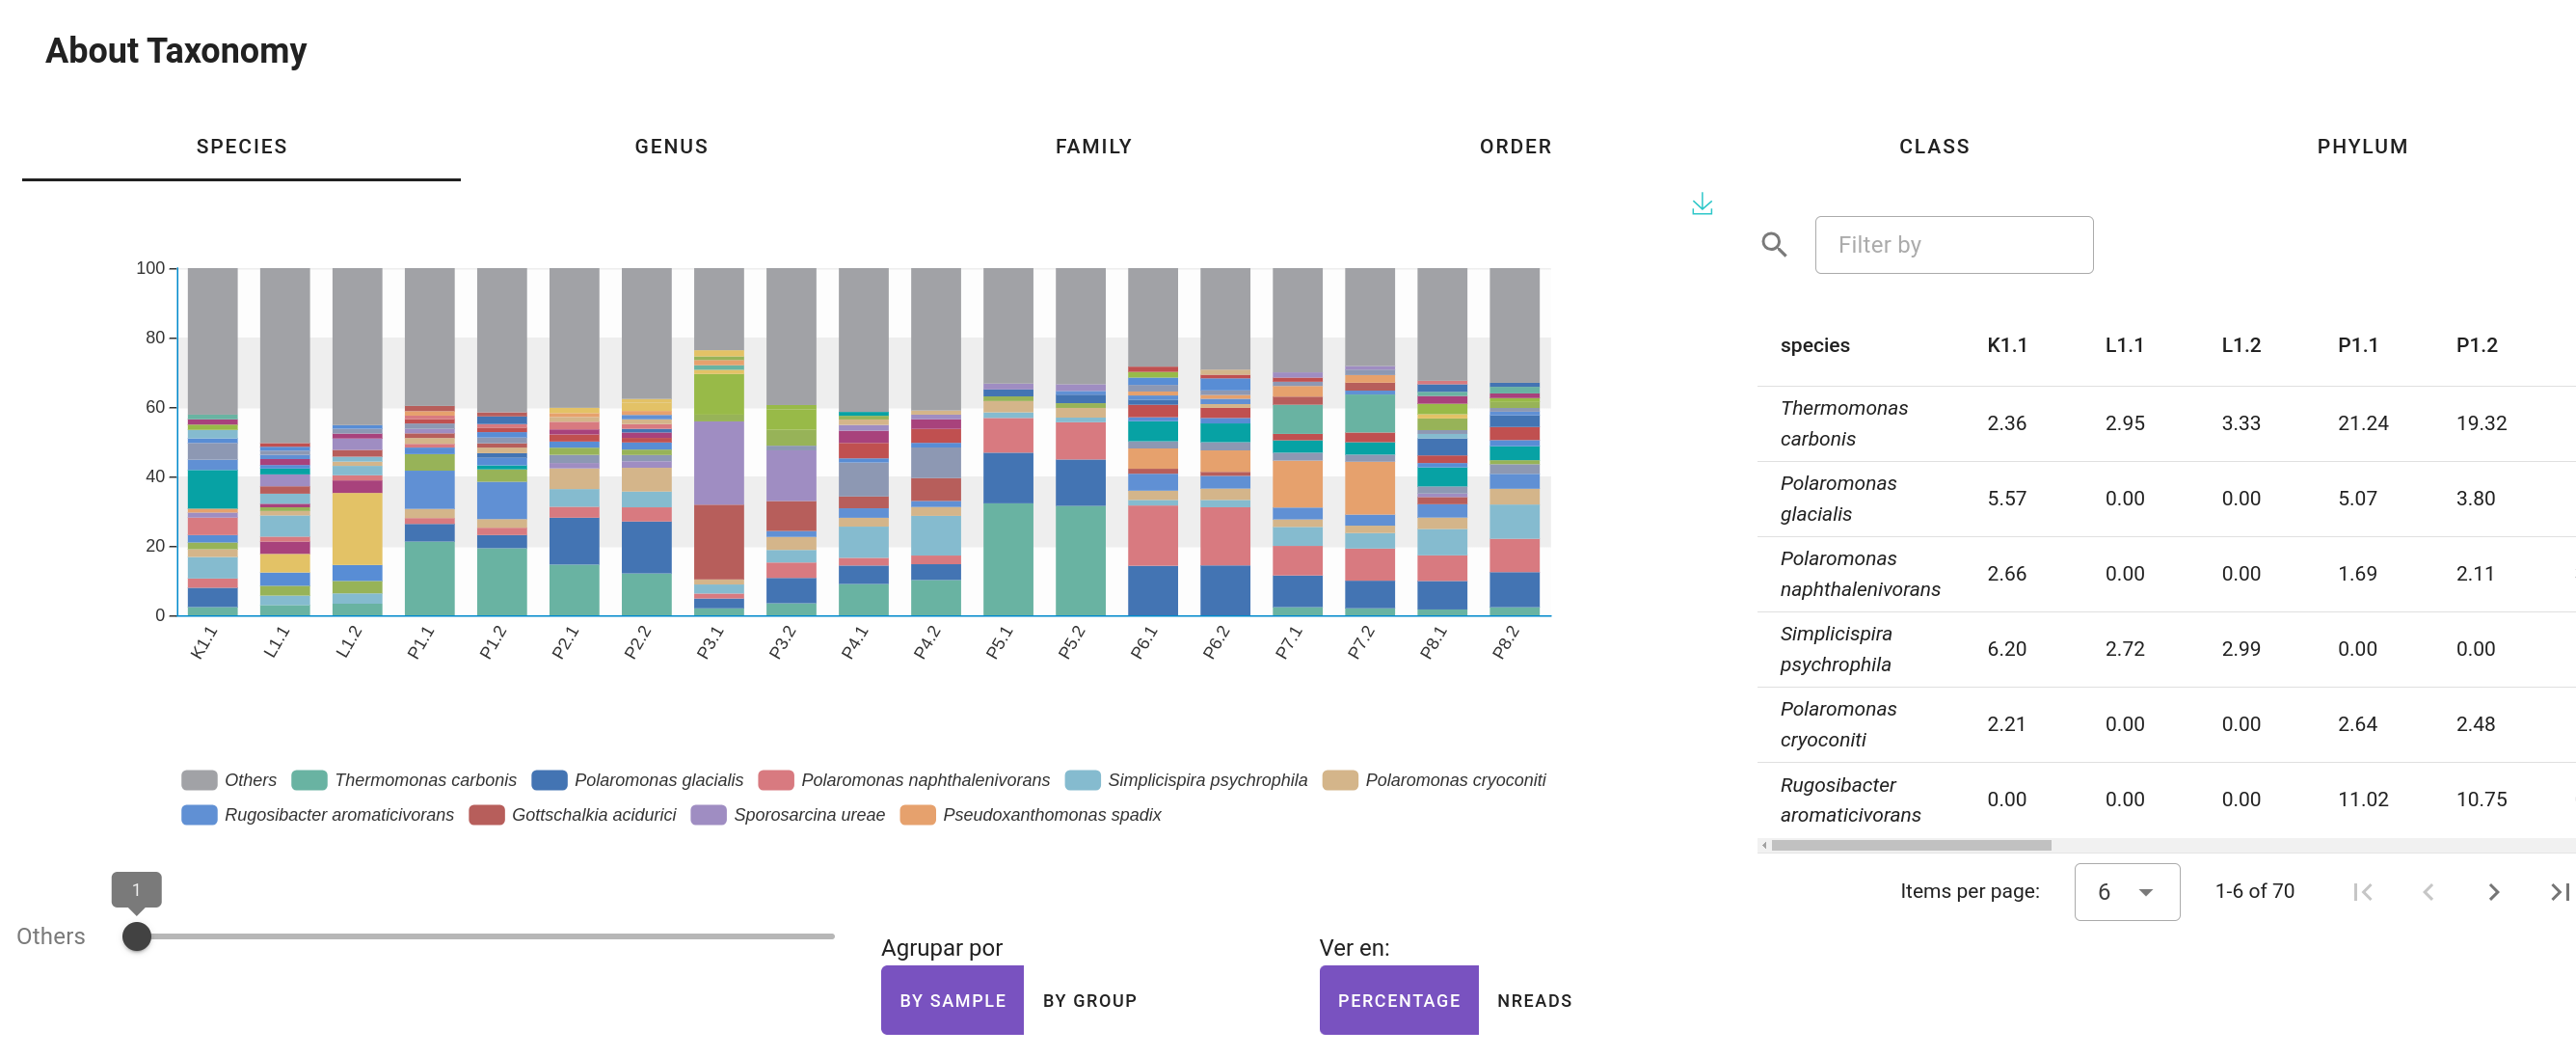
\includegraphics[width=1\linewidth]{images/app/results/taxonomy.png}
    % \captionsetup{justification=raggedright, width=0.45\linewidth, singlelinecheck=off}

    % \captionsetup{width=0.45\linewidth}
    \caption{Vista de asignación taxonómica (resultados)}
    \label{fig:app-results-taxonomy}
\end{figure}

% En el lado derecho, hay una tabla que permite visualizar el detalle de la información presentada en el gráfico. 
% Se puede visualizar además un campo de texto que permite al usuario buscar una taxonomía en especifico y visualizar su abundancia o cantidad de lecturas en todas las muestras.

En caso de que la pantalla tenga una resolución menor a 992px la tabla y gráfico se desplegarán uno debajo del otro(Figura~\ref{fig:app-results-taxonomy-small-dev}).
\begin{figure}[H]
    \centering
    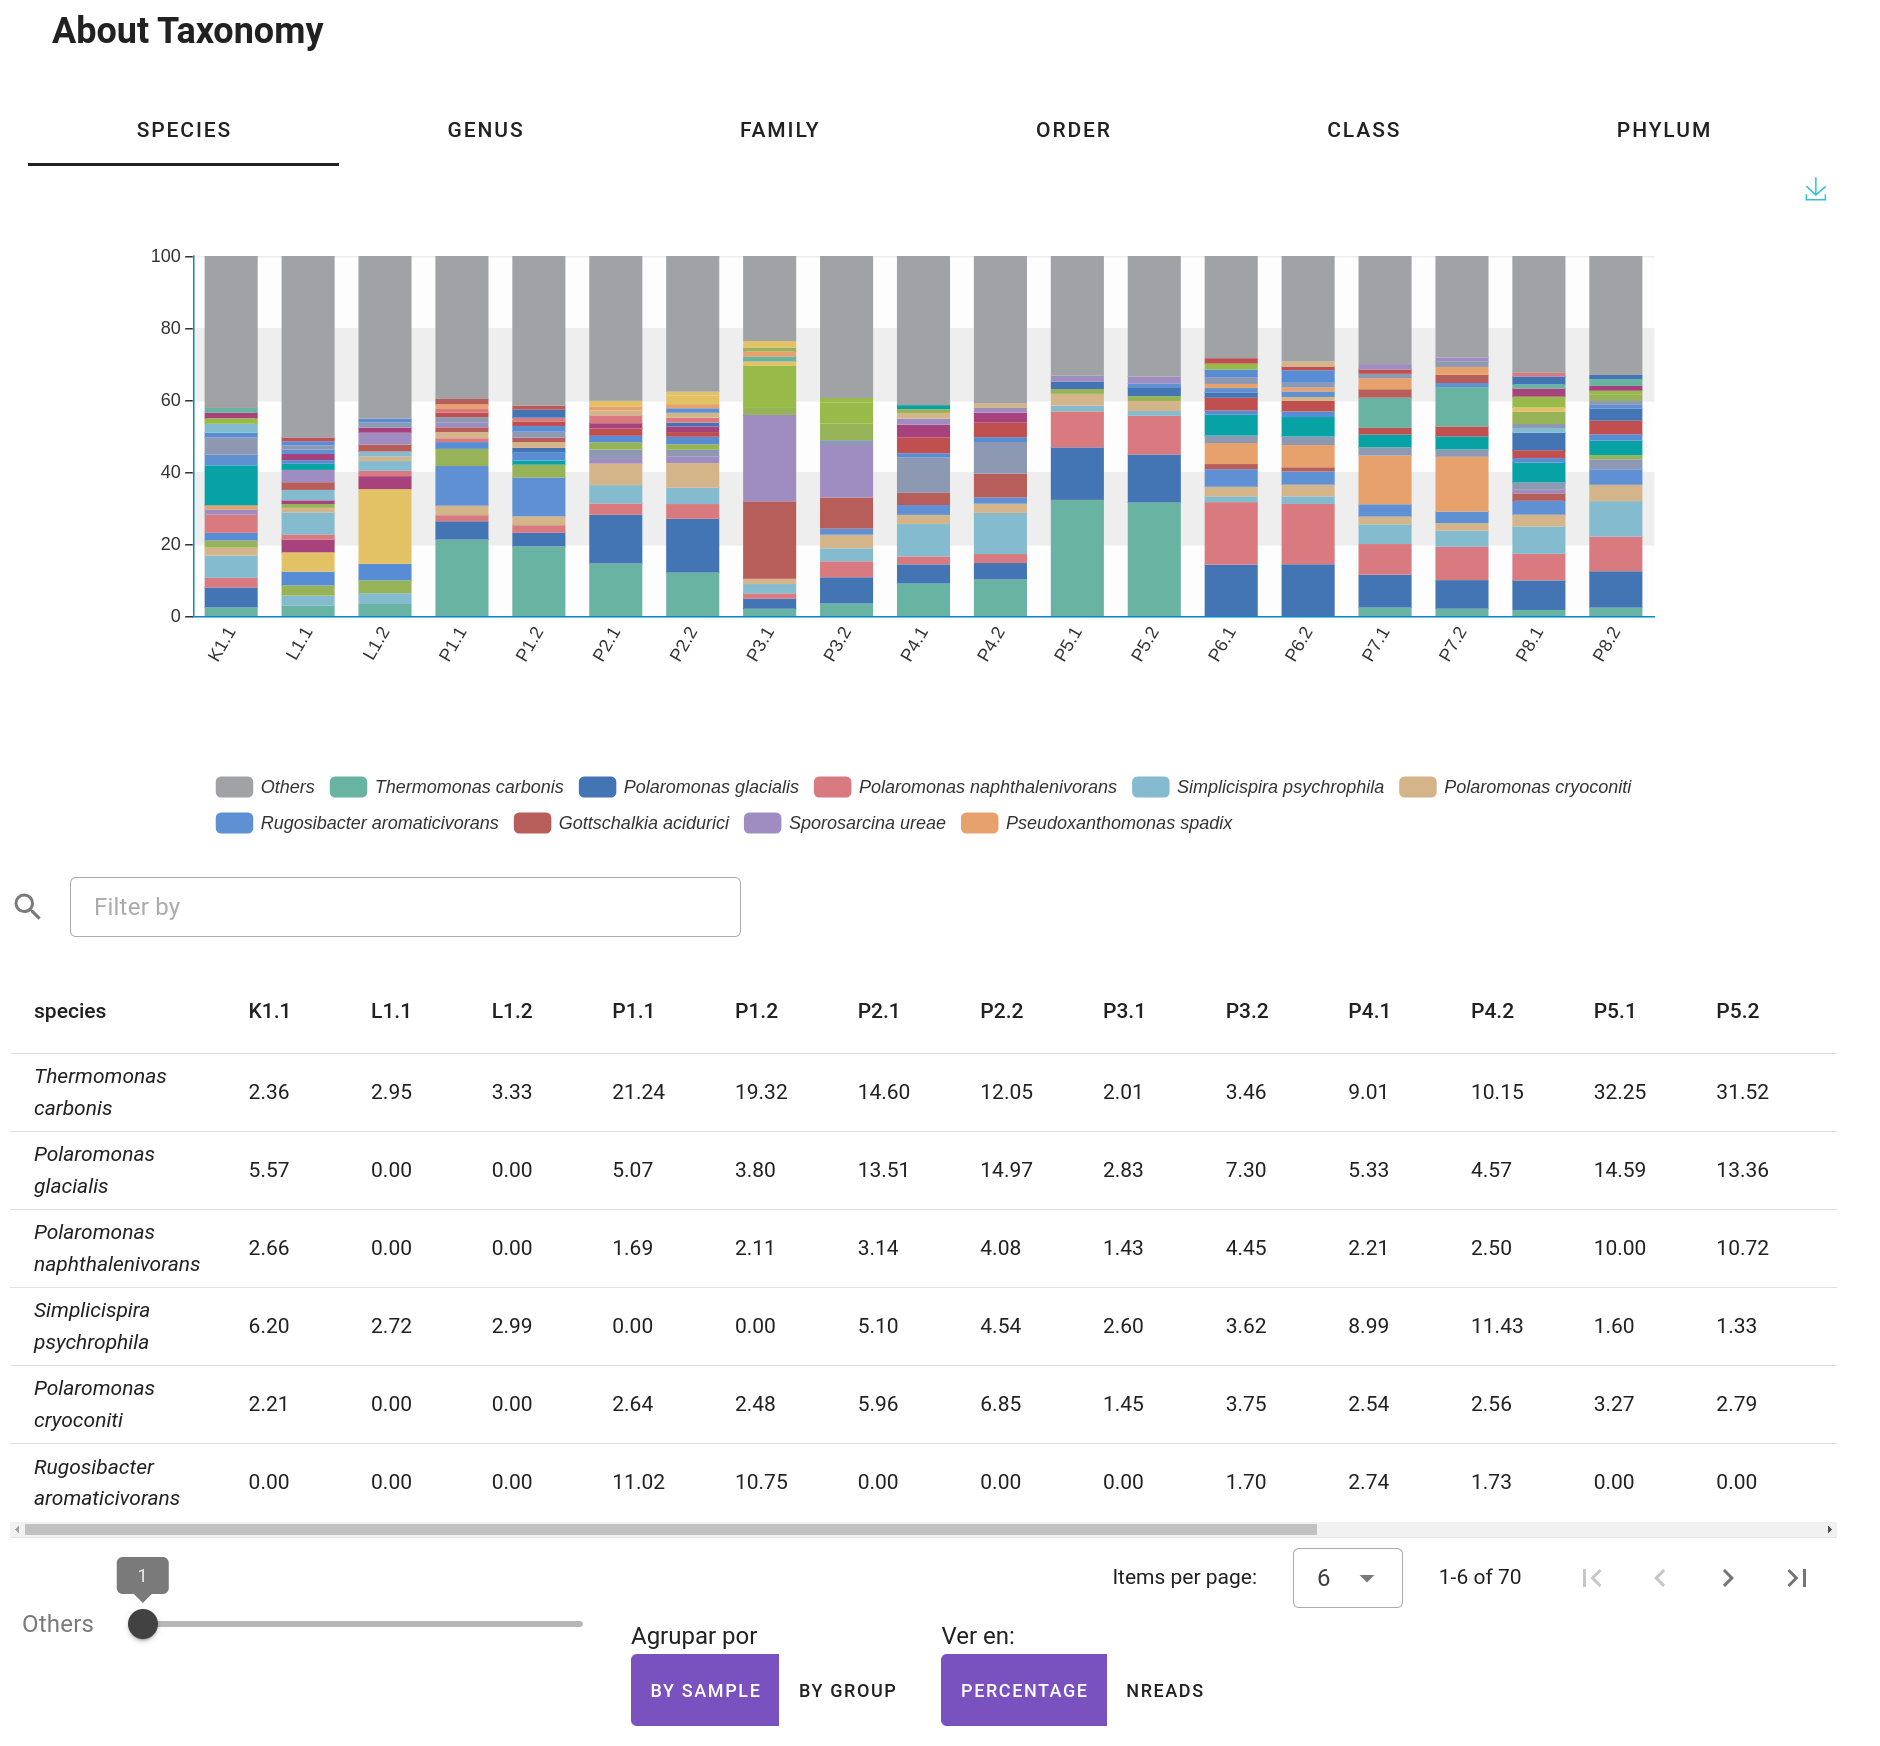
\includegraphics[width=0.8\linewidth]{images/app/results/taxonomy_small_dev.png}
    % \captionsetup{justification=raggedright, width=0.45\linewidth, singlelinecheck=off}

    % \captionsetup{width=0.45\linewidth}
    \caption{Estadisticas básicas (resultados)}
    \label{fig:app-results-taxonomy-small-dev}
\end{figure}

Ambos componentes, la tabla y el gráfico de barras apiladas se ajustan automáticamente para presentar la información requerida por el usuario, es decir, cada vez que el usuario selecciona una nueva categoría taxonómica en las pestañas, se vuelve a generar la información proporcionando una visualización clara y detallada de los datos.







% El usuario puede modificar la visualización de la información en el gráfico de barras apiladas y tabla a través de las pestañas que se encuentran en la parte superior del gráfico 
En la Figura~\ref{fig:app-results-taxonomy-order} el usuario seleccionó la pestaña de orden, por lo que se visualiza la información de la taxonomía en la categoría de orden.
\begin{figure}[H]
    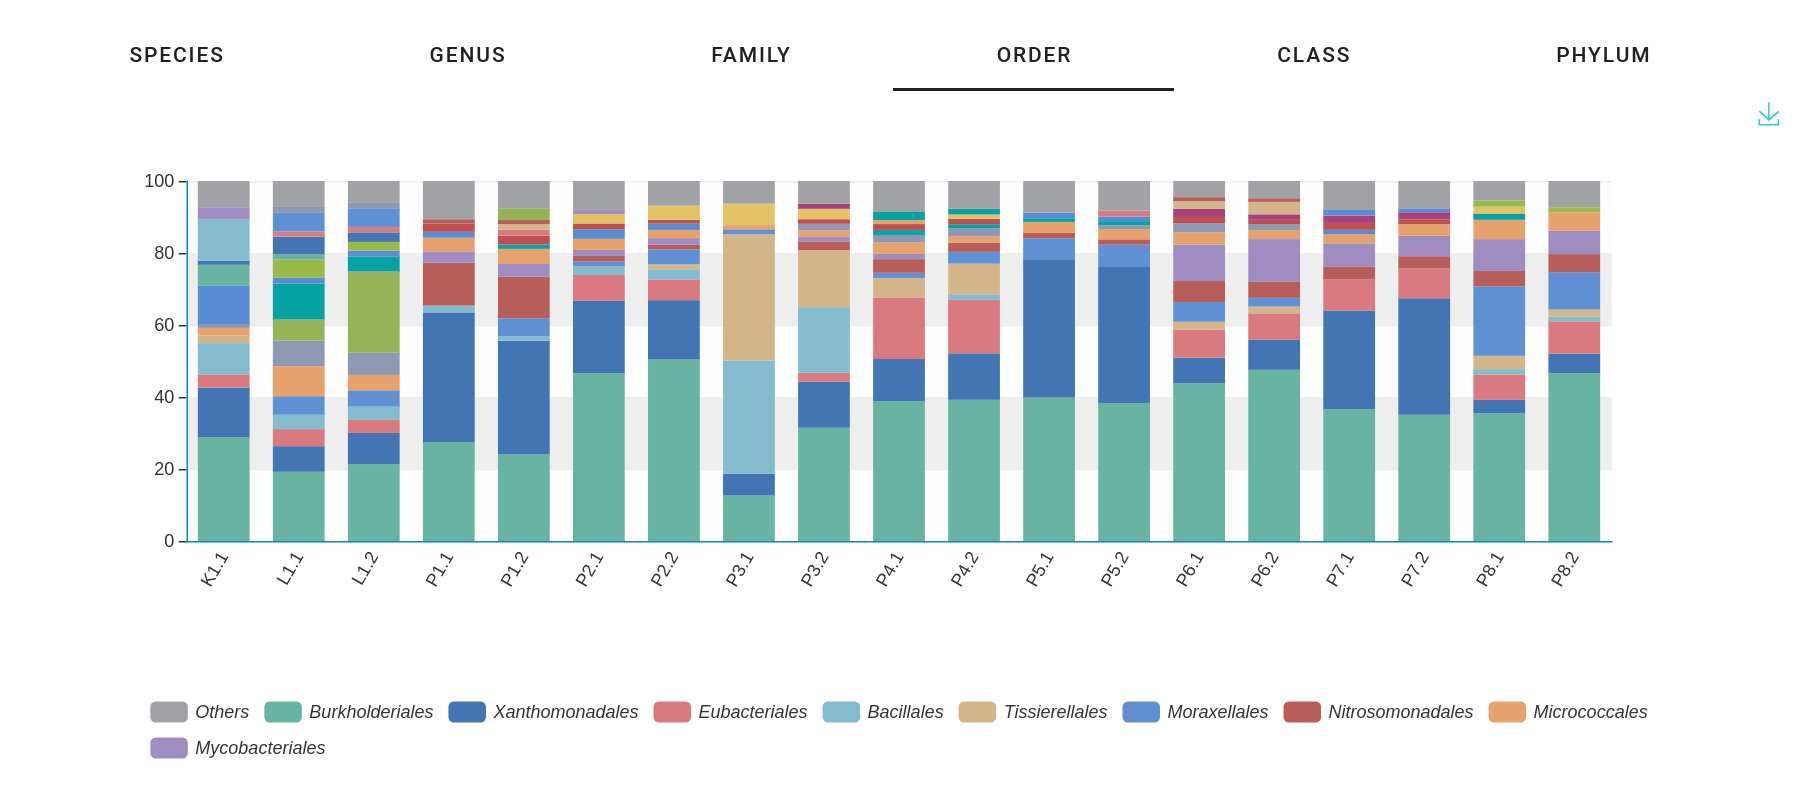
\includegraphics[width=1\linewidth]{images/app/results/taxonomy_order.png}
    % \captionsetup{justification=raggedright, width=0.45\linewidth, singlelinecheck=off}

    % \captionsetup{width=0.45\linewidth}
    \caption{Vista de asignación taxonómica en categoría de orden (stacked plot)}
    \label{fig:app-results-taxonomy-order}
\end{figure}



% \begin{figure}[H]
%     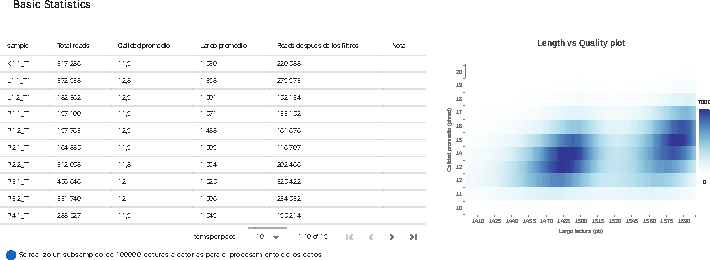
\includegraphics[width=1\linewidth]{images/app/results/basicStatistics.png}
%     % \captionsetup{justification=raggedright, width=0.45\linewidth, singlelinecheck=off}

%     % \captionsetup{width=0.45\linewidth}
%     \caption{Estadisticas básicas (resultados)}
%     \label{fig:app-results-taxonomicAssig-group-perc}
% \end{figure}




El usuario también puede modificar la información de la tabla y gráfico utilizando los botones que se encuentran en la parte inferior del gráfico. 
Pudiendo visualizar la información en porcentaje o en cantidad de lecturas~\ref{fig:app-results-taxonomy-sample-nreads}, como también pudiendo agrupar las muestras por grupo~\ref{fig:app-results-taxonomy-groups-perc}.
\begin{figure}[H]
    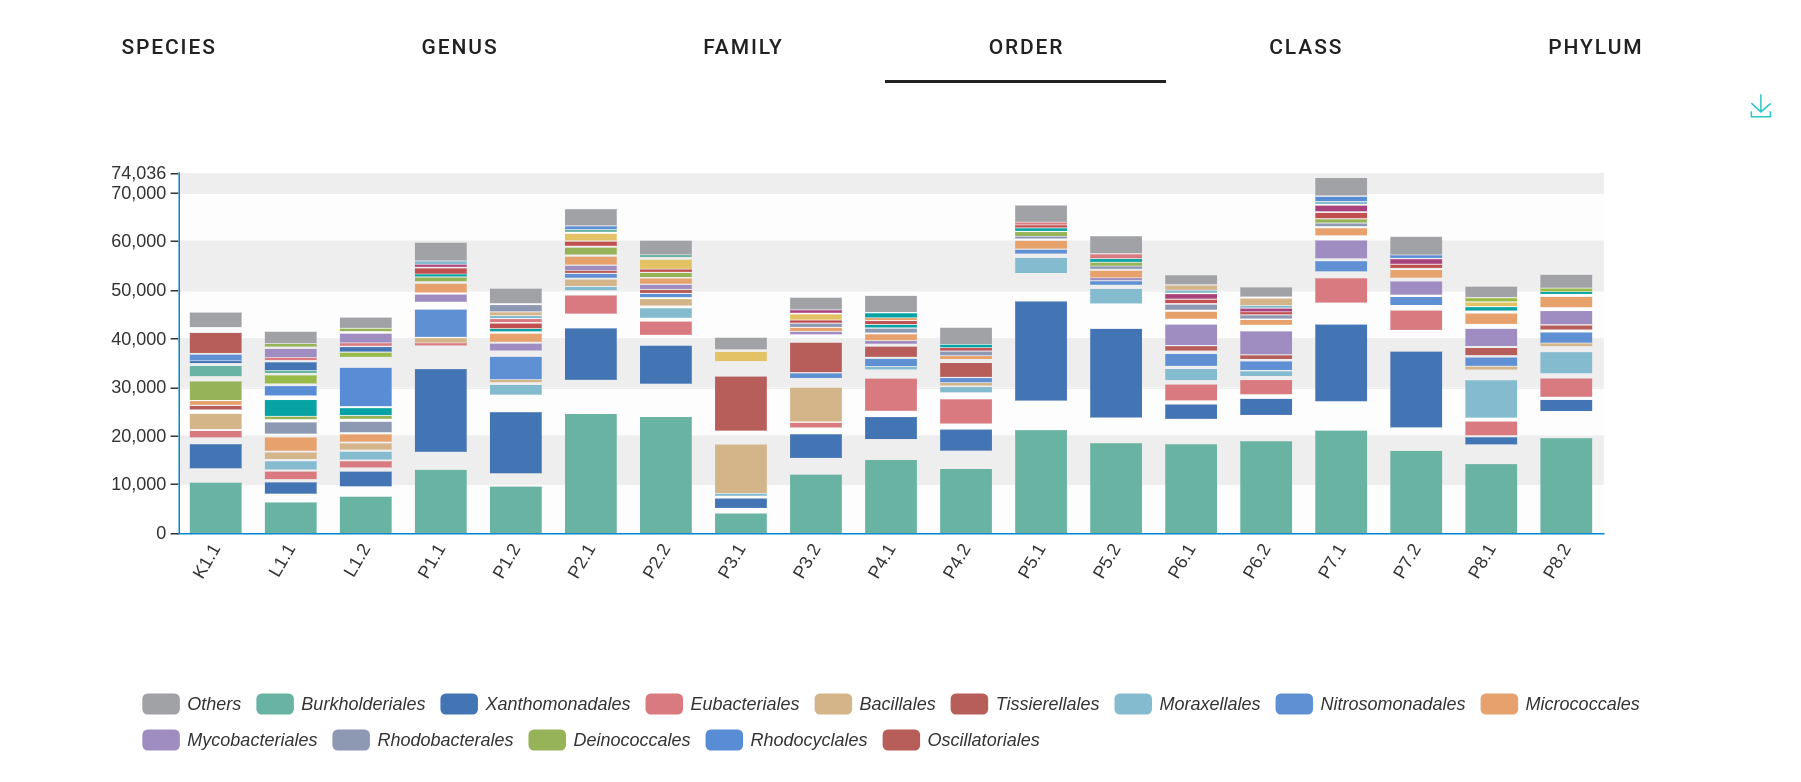
\includegraphics[width=1\linewidth]{images/app/results/taxonomy_sample_nreads.png}
    % \captionsetup{justification=raggedright, width=0.45\linewidth, singlelinecheck=off}

    % \captionsetup{width=0.45\linewidth}
    \caption{Taxonomias por muestra utilizando cantidad de lecturas}
    \label{fig:app-results-taxonomy-sample-nreads}
\end{figure}

\begin{figure}[H]
    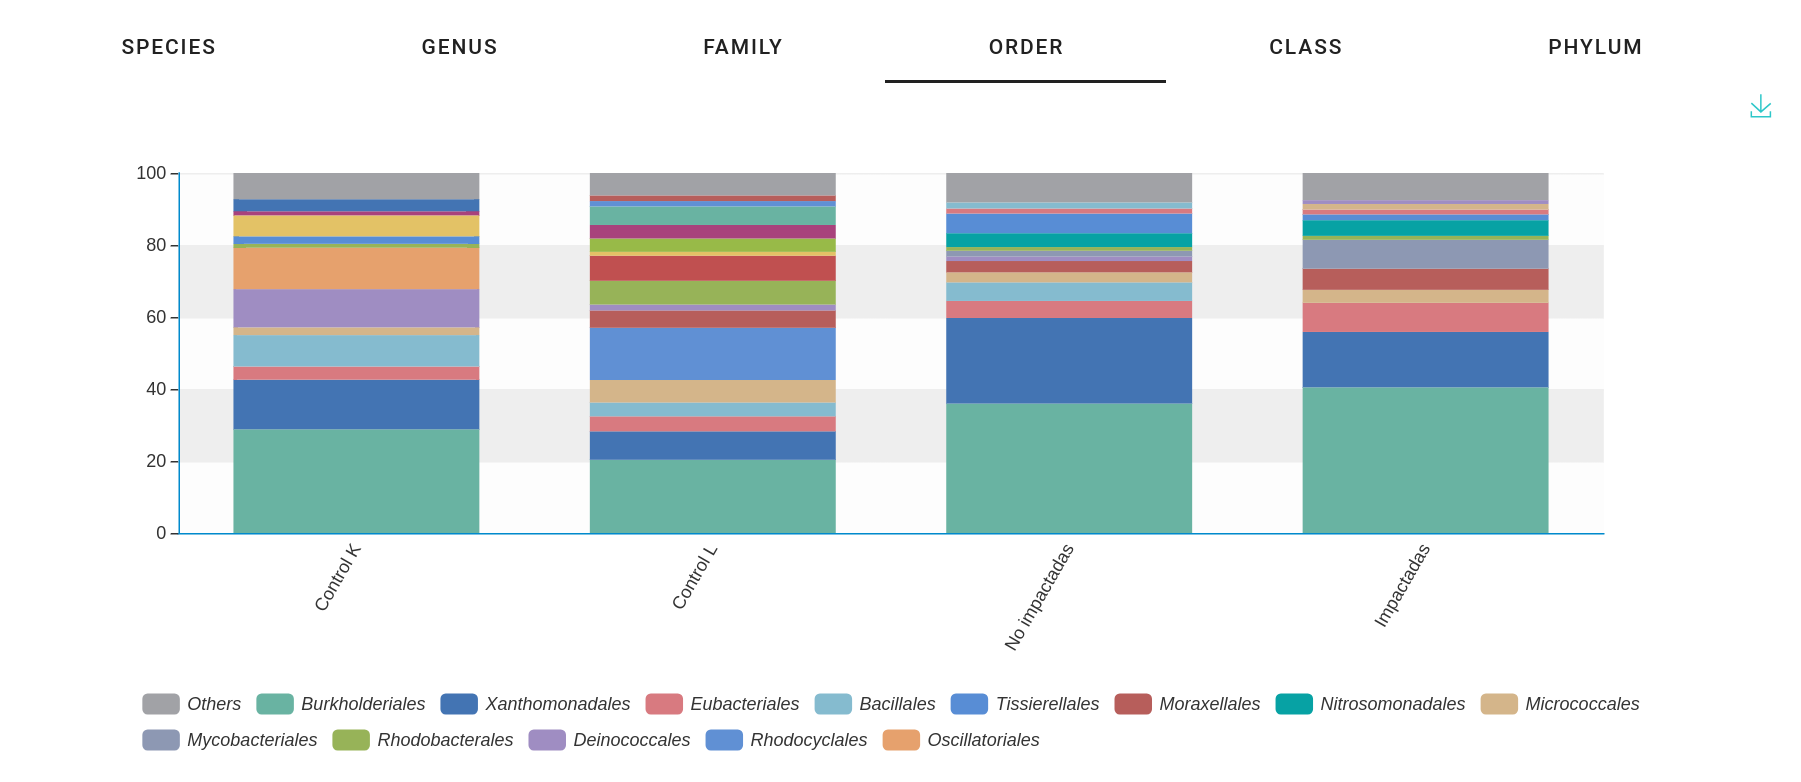
\includegraphics[width=1\linewidth]{images/app/results/taxonomy_grooups_perc.png}
    % \captionsetup{justification=raggedright, width=0.45\linewidth, singlelinecheck=off}

    % \captionsetup{width=0.45\linewidth}
    \caption{Taxonomias por grupo utilizando valor porcentual}
    \label{fig:app-results-taxonomy-groups-perc}
\end{figure}


De igual forma el usuario puede posicionar el mouse sobre alguna barra del gráfico o sobre alguna taxonomía de la leyenda y destacar esa taxonomía en todas las muestras y visualizar el porcentaje o cantidad de lecturas en la muestra que el mouse se encuentra posicionado (Figura~\ref{fig:app-results-taxonomicAssig-others}).
\begin{figure}[H]
    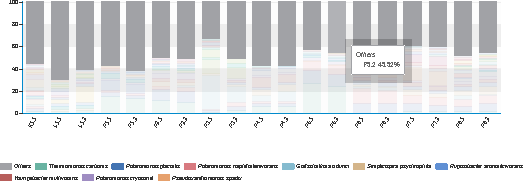
\includegraphics[width=1\linewidth]{images/app/results/taxonomy_others.pdf}
    % \captionsetup{justification=raggedright, width=0.45\linewidth, singlelinecheck=off}

    % \captionsetup{width=0.45\linewidth}
    \caption{Taxonomía por muestra: Destacar taxonomía en todas las muestras}
    \label{fig:app-results-taxonomicAssig-others}
\end{figure}


La tabla de taxonomías presenta un campo de búsqueda en la parte superior que permite al usuario filtrar la tabla por una taxonomía en especifico (Figura~\ref{fig:app-results-taxonomy-search}).
En el ejemplo se busca la palabra \textit{Polar} por lo que aparecen todas taxonomías que contienen esta palabra en su nombre.
\begin{figure}[H]
    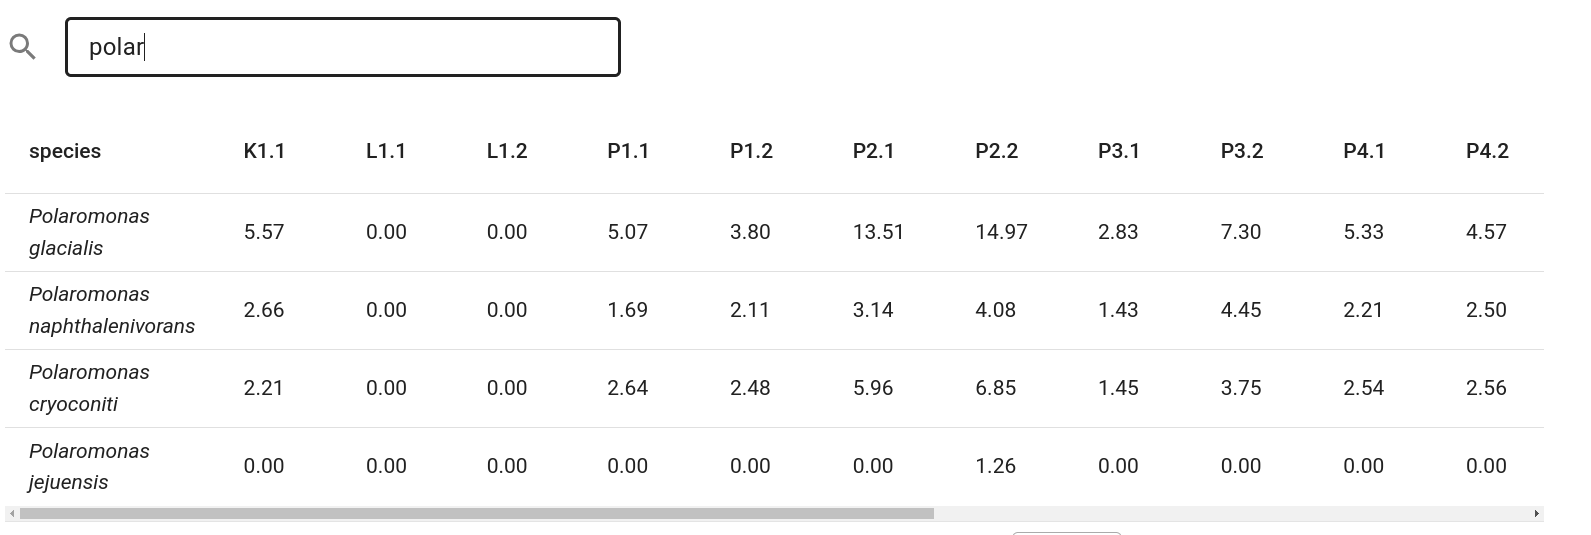
\includegraphics[width=0.9\linewidth]{images/app/results/taxonomy_search.png}
    % \captionsetup{justification=raggedright, width=0.45\linewidth, singlelinecheck=off}

    % \captionsetup{width=0.45\linewidth}
    \caption{Filtro de resultados en tabla de asignación taxonómica}
    \label{fig:app-results-taxonomy-search}
\end{figure}

\subsection{Similitud entre las muestras}
Esta sección representa las taxonomías compartidas por las muestras mediante un gráfico circular de anillos jerarquicos. 
Cada nivel del gráfico representa una categoría taxonómica, siendo la más interna especie, y la más externa filo.
Mientras más grande el diamentro del anillo en el gráfico, mayor es la presencia de esa taxonomía en las muestras.

Las taxonomías presentadas incluyen todas las taxonomías con abundancia mayor al 1\% y que estan presentes en todas las muestras del grupo.
El porcentaje presentado corresponde el porcentaje de todas las lecturas en el grupo graficado.


A continuación se presenta un ejemplo de como se visualiza el gráfico circular de anillos jerarquicos para dos grupos(Figura~\ref{fig:app-results-core}).
\begin{figure}[H]
    \centering
    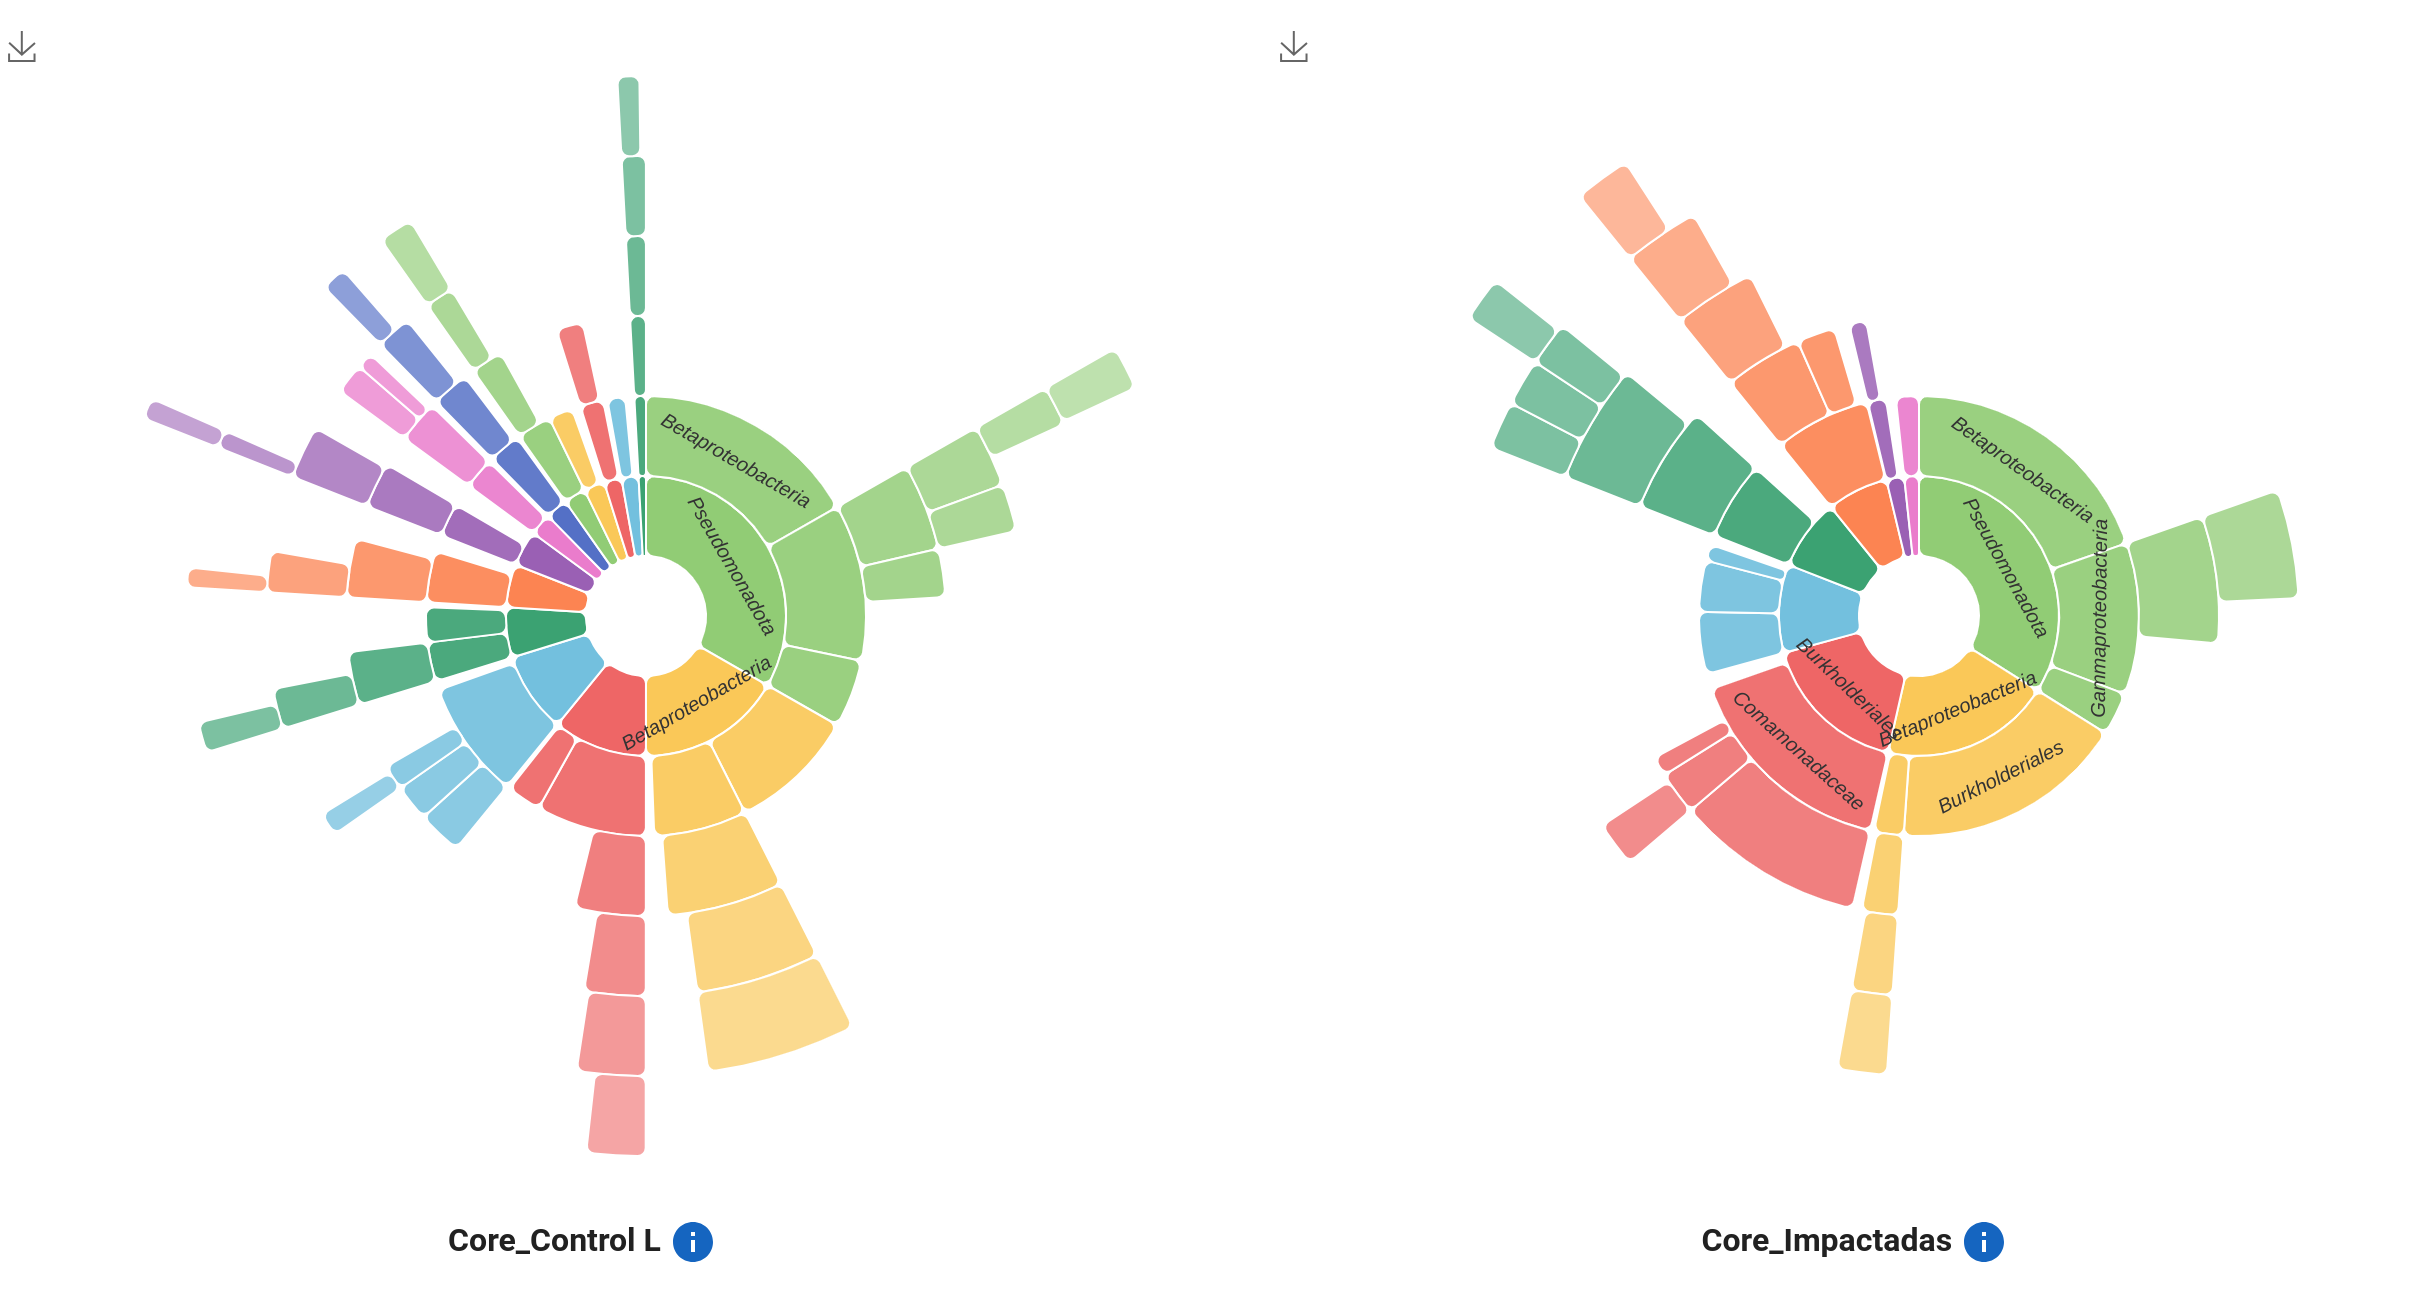
\includegraphics[width=0.8\linewidth]{images/app/results/core.png}
    % \captionsetup{justification=raggedright, width=0.45\linewidth, singlelinecheck=off}

    % \captionsetup{width=0.45\linewidth}
    \caption{Gráfico de similitud  (resultados)}
    \label{fig:app-results-core}
\end{figure}

En esta sección se puede presentar un solo gráfico de las taxonomías compartidas entre todas las muestras, y en el caso de que el usuario haya ingresado grupos, se desplegaran además los gráficos por cada grupo, como se visualiza en la Figura~\ref{fig:app-results-core}.

En la parte inferior del gráfico, al lado derecho de la leyenda se puede visualizar un icono, el cual al posicionarse sobre el, va a mostrar las muestras utilizadas para generar el gráfico(Figura~\ref{fig:app-results-core-tooltip}).

\begin{figure}[H]
    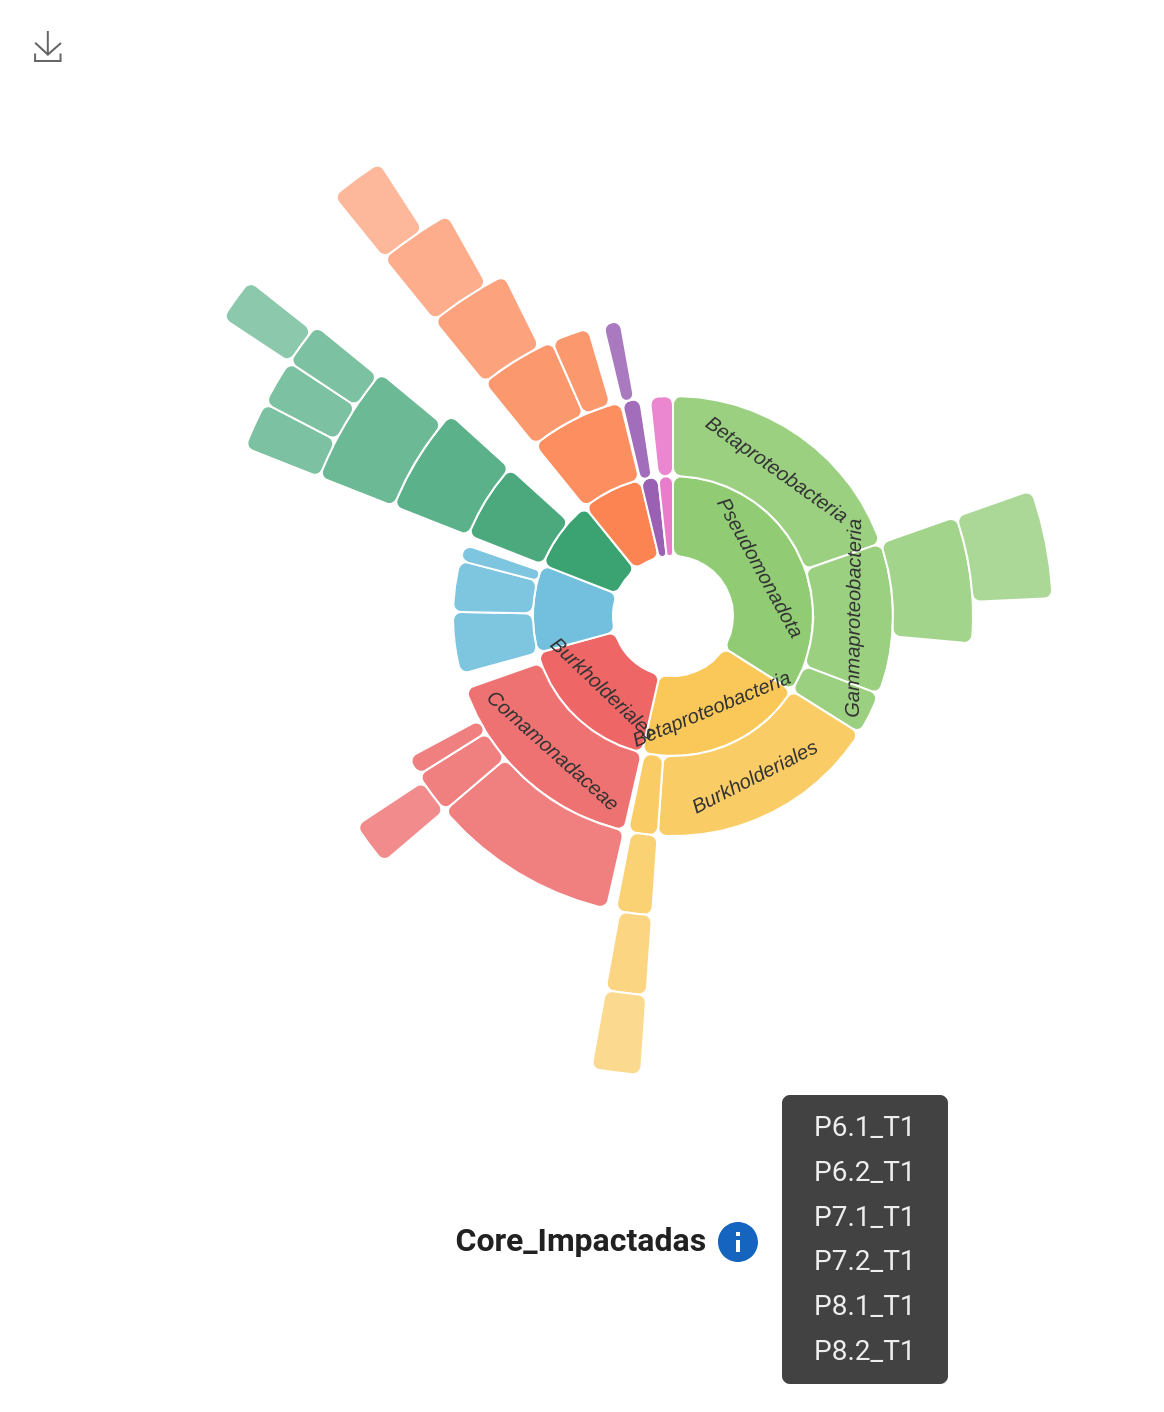
\includegraphics[width=0.8\linewidth]{images/app/results/core_tooltip.png}
    % \captionsetup{justification=raggedright, width=0.45\linewidth, singlelinecheck=off}

    % \captionsetup{width=0.45\linewidth}
    \caption{Gráfico de similitud: Tooltip asociado a las muestras (resultados)}
    \label{fig:app-results-core-tooltip}
\end{figure}

\subsection{Indices de diversidad}

En caso de que el usuario hubiera ingresado grupos al inicio del proyecto y hubiera activado los análisis de índices de diversidad, se podrá visualizar tres gráficos boxplot, uno por cada índice de diversidad (Shannon, Simpson y Chao2). En caso de que el usuario no haya ingresado grupos, esta sección no se desplegará en la plataforma.

A continuación se presenta un ejemplo de la visualización de esta sección en la plataforma:



\subsection{Predicción funcional}
Al igual que en la sección de asignación taxonómica, en la parte superior se pueden visualizar tres pestañas \textit{EC, KO y Pathways} que representan cada categoría funcional. Por defecto se presenta la información para la categoría de \textit{Pathways}.

En la parte inferior izquierda se puede visualizar una tabla con la información de la predicción funcional obtenida mediante PICRUSt2 (EC, KO y Pathways) para cada muestra. 
En la parte superior de la tabla se puede visualizar un campo de texto de búsqueda con el cual el usuario puede filtrar la información de la tabla.

En el lado derecho de la sección, en caso de que el usuario hubiera ingresado grupos, se puede ver un gráfico de barras horizontales que muestra los pathways con diferencias significativas entre los grupos (información obtenida mediante LEfSe). 
En caso de que no se haya ingresado información de grupos, solo se desplegará la tabla.

Al igual que en la sección de asignación taxonómica el usuario puede interactuar con las pestañas modificando el contenido de las tablas mediante la selección de las pestañas.


\begin{figure}[H]
    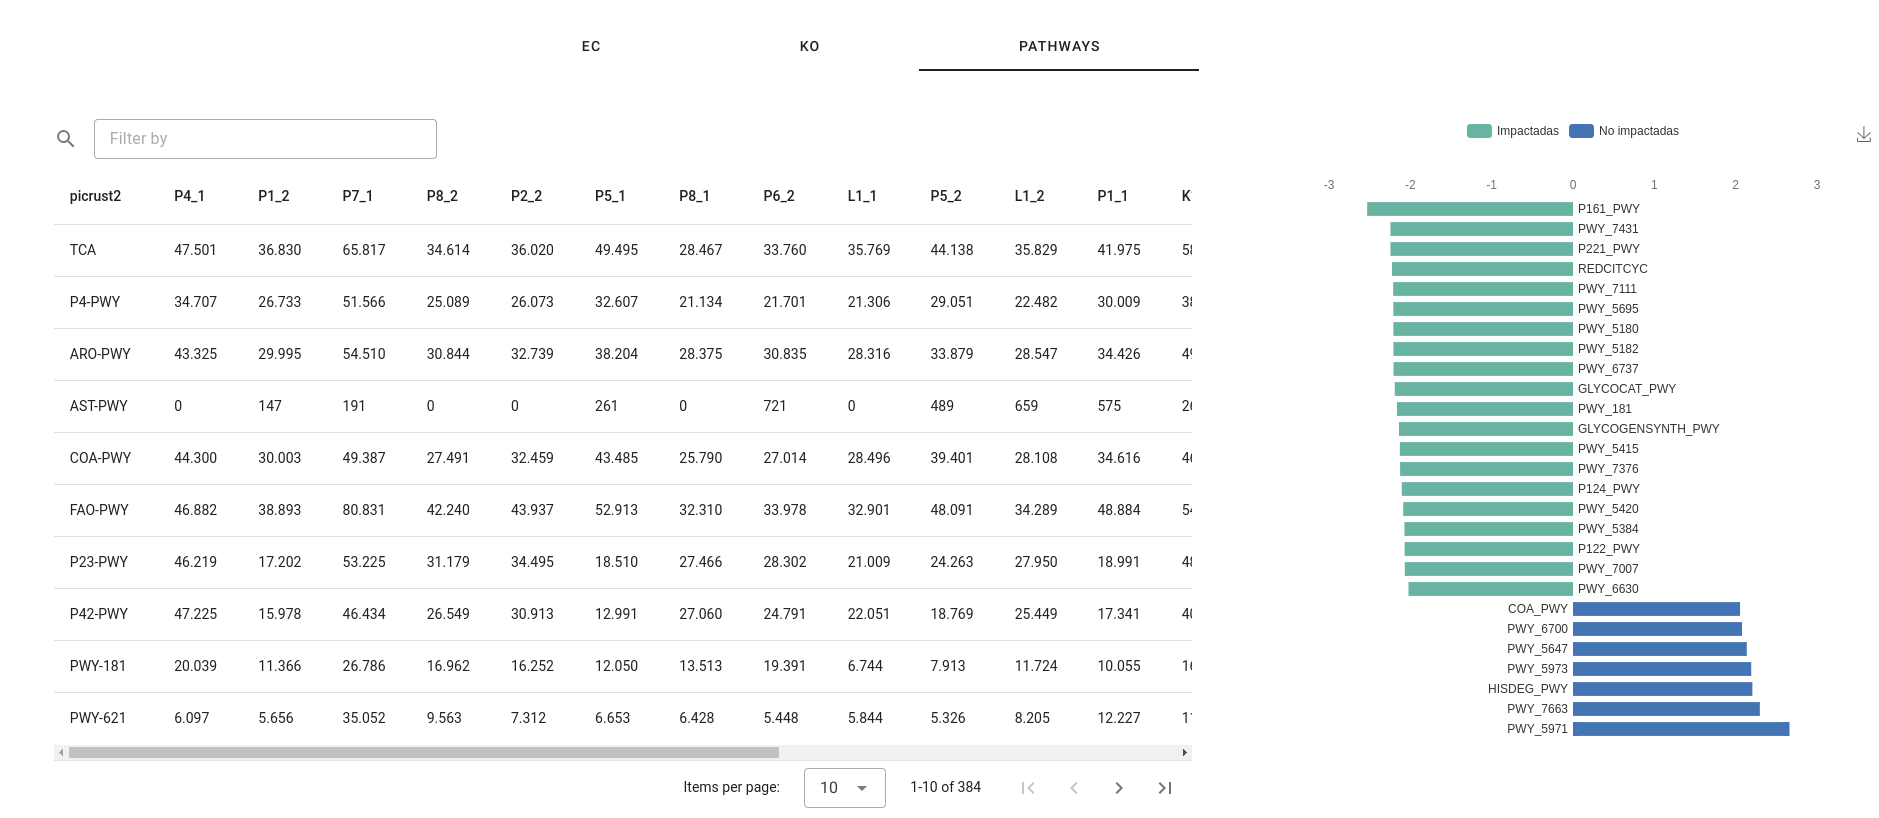
\includegraphics[width=1\linewidth]{images/app/results/functinoal_pred.png}
    % \captionsetup{justification=raggedright, width=0.45\linewidth, singlelinecheck=off}

    % \captionsetup{width=0.45\linewidth}
    \caption{Resultados de predicción funcional: Tabla obtenida mediante PICRUSt2 y gráficod de diferencias significativas obtenido mediante LefSE}
    \label{fig:app-results-functional-pred}
\end{figure}
\subsubsection{Descarga de los resultados}
En la parte superior derecha de la sección de resultados, se encuentra un botón con el texto \textit{Download data}. 
Al hacer click en este botón se descargará un archivo comprimido con toda los resultados generados por el pipeline.
A continuación se detallan los archivos:
\begin{itemize}
    \item CSV de asignación taxonomica por muestra y por grupo (en caso de ingresarse), y por porcentaje y cantidad de lecturas
    \item CSV de predicción funcional (EC, KO y pathways), en caso de haber seleccionado predicción funcional dentro de los análisis.
    \item CSV con los valores del cálculo de los indices de diversidad
    % \item \hl{PDF con los gráficos de barras apiladas, Sunburst y boxplot}
    % \item \hl{Archivo de texto con la información del pipeline (versión, parámetros, etc)}
\end{itemize}


\begin{figure}[H]
    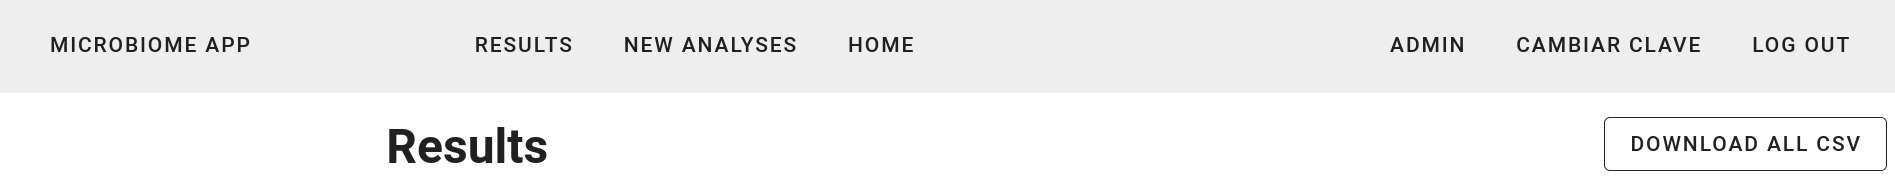
\includegraphics[width=1\linewidth]{images/app/donwload_button.png}
    % \captionsetup{justification=raggedright, width=0.45\linewidth, singlelinecheck=off}

    % \captionsetup{width=0.45\linewidth}
    \caption{Gráfico de similitud: Tooltip asociado a las muestras (resultados)}
    \label{fig:app-download-button}
\end{figure}

% \begin{figure}[H]
%     \includegraphics[width=1\linewidth]{images/app/results/downloadbutton.png}
%     % \captionsetup{justification=raggedright, width=0.45\linewidth, singlelinecheck=off}

%     % \captionsetup{width=0.45\linewidth}
%     \caption{Botón de descarga de resultados(resultados)}
%     \label{fig:app-results-download}
% \end{figure}

\subsection{Integración del flujo de trabajo y aplicación web}

Se diseñó una base de datos no relacional utilizando PostgreSQL.
Esta base de datos permite almacenar la información de los proyectos subidos por el usuario en la plataforma web y los resultados obtenidos al ejecutar el flujo de trabajo.
La base de datos funciona como intermedio entre el flujo de trabajo y la base de datos, permitiendo que la aplicación web escriba la metadata asociada al proyecto para que el flujo de trabajo pueda ejecutarse, y permitiendo además que la aplicación web pueda leer los resultados escritos por el flujo de trabajo, para poder convertir esta información en tablas y gráficos que permitan al usuario visualizar los resultados de manera sencilla.

La base de datos esta compuesta por siete tablas:
\begin{itemize}
    \item PlatformRoles: Almacena los roles de la plataforma (admin, basic user).
    \item Users: Almacena la información de los usuarios registrados en la plataforma.
    \item Projects: Almacena la información de los proyectos subidos por los usuarios.
    \item ProjectRoles: Almacena los roles de los usuarios dentro de los proyectos. Esto permite que un projecto y sus resultados puedan ser visualizados por varios usuarios a la vez.
    \item ProjectRolesUsers: Almacena la relación entre los usuarios y los roles de los proyectos. Permitiendo a los usuarios tener diferentes roles en diferentes proyectos (solo lectura, edición, eliminar).
    \item Results: Almacena los resultados obtenidos en la ejecución del flujo de trabajo.
    \item PipelineDefaultParams: Almacena los parámetros por defecto de cada versión del flujo de trabajo.
\end{itemize}

\begin{figure}[H]
    \centering
    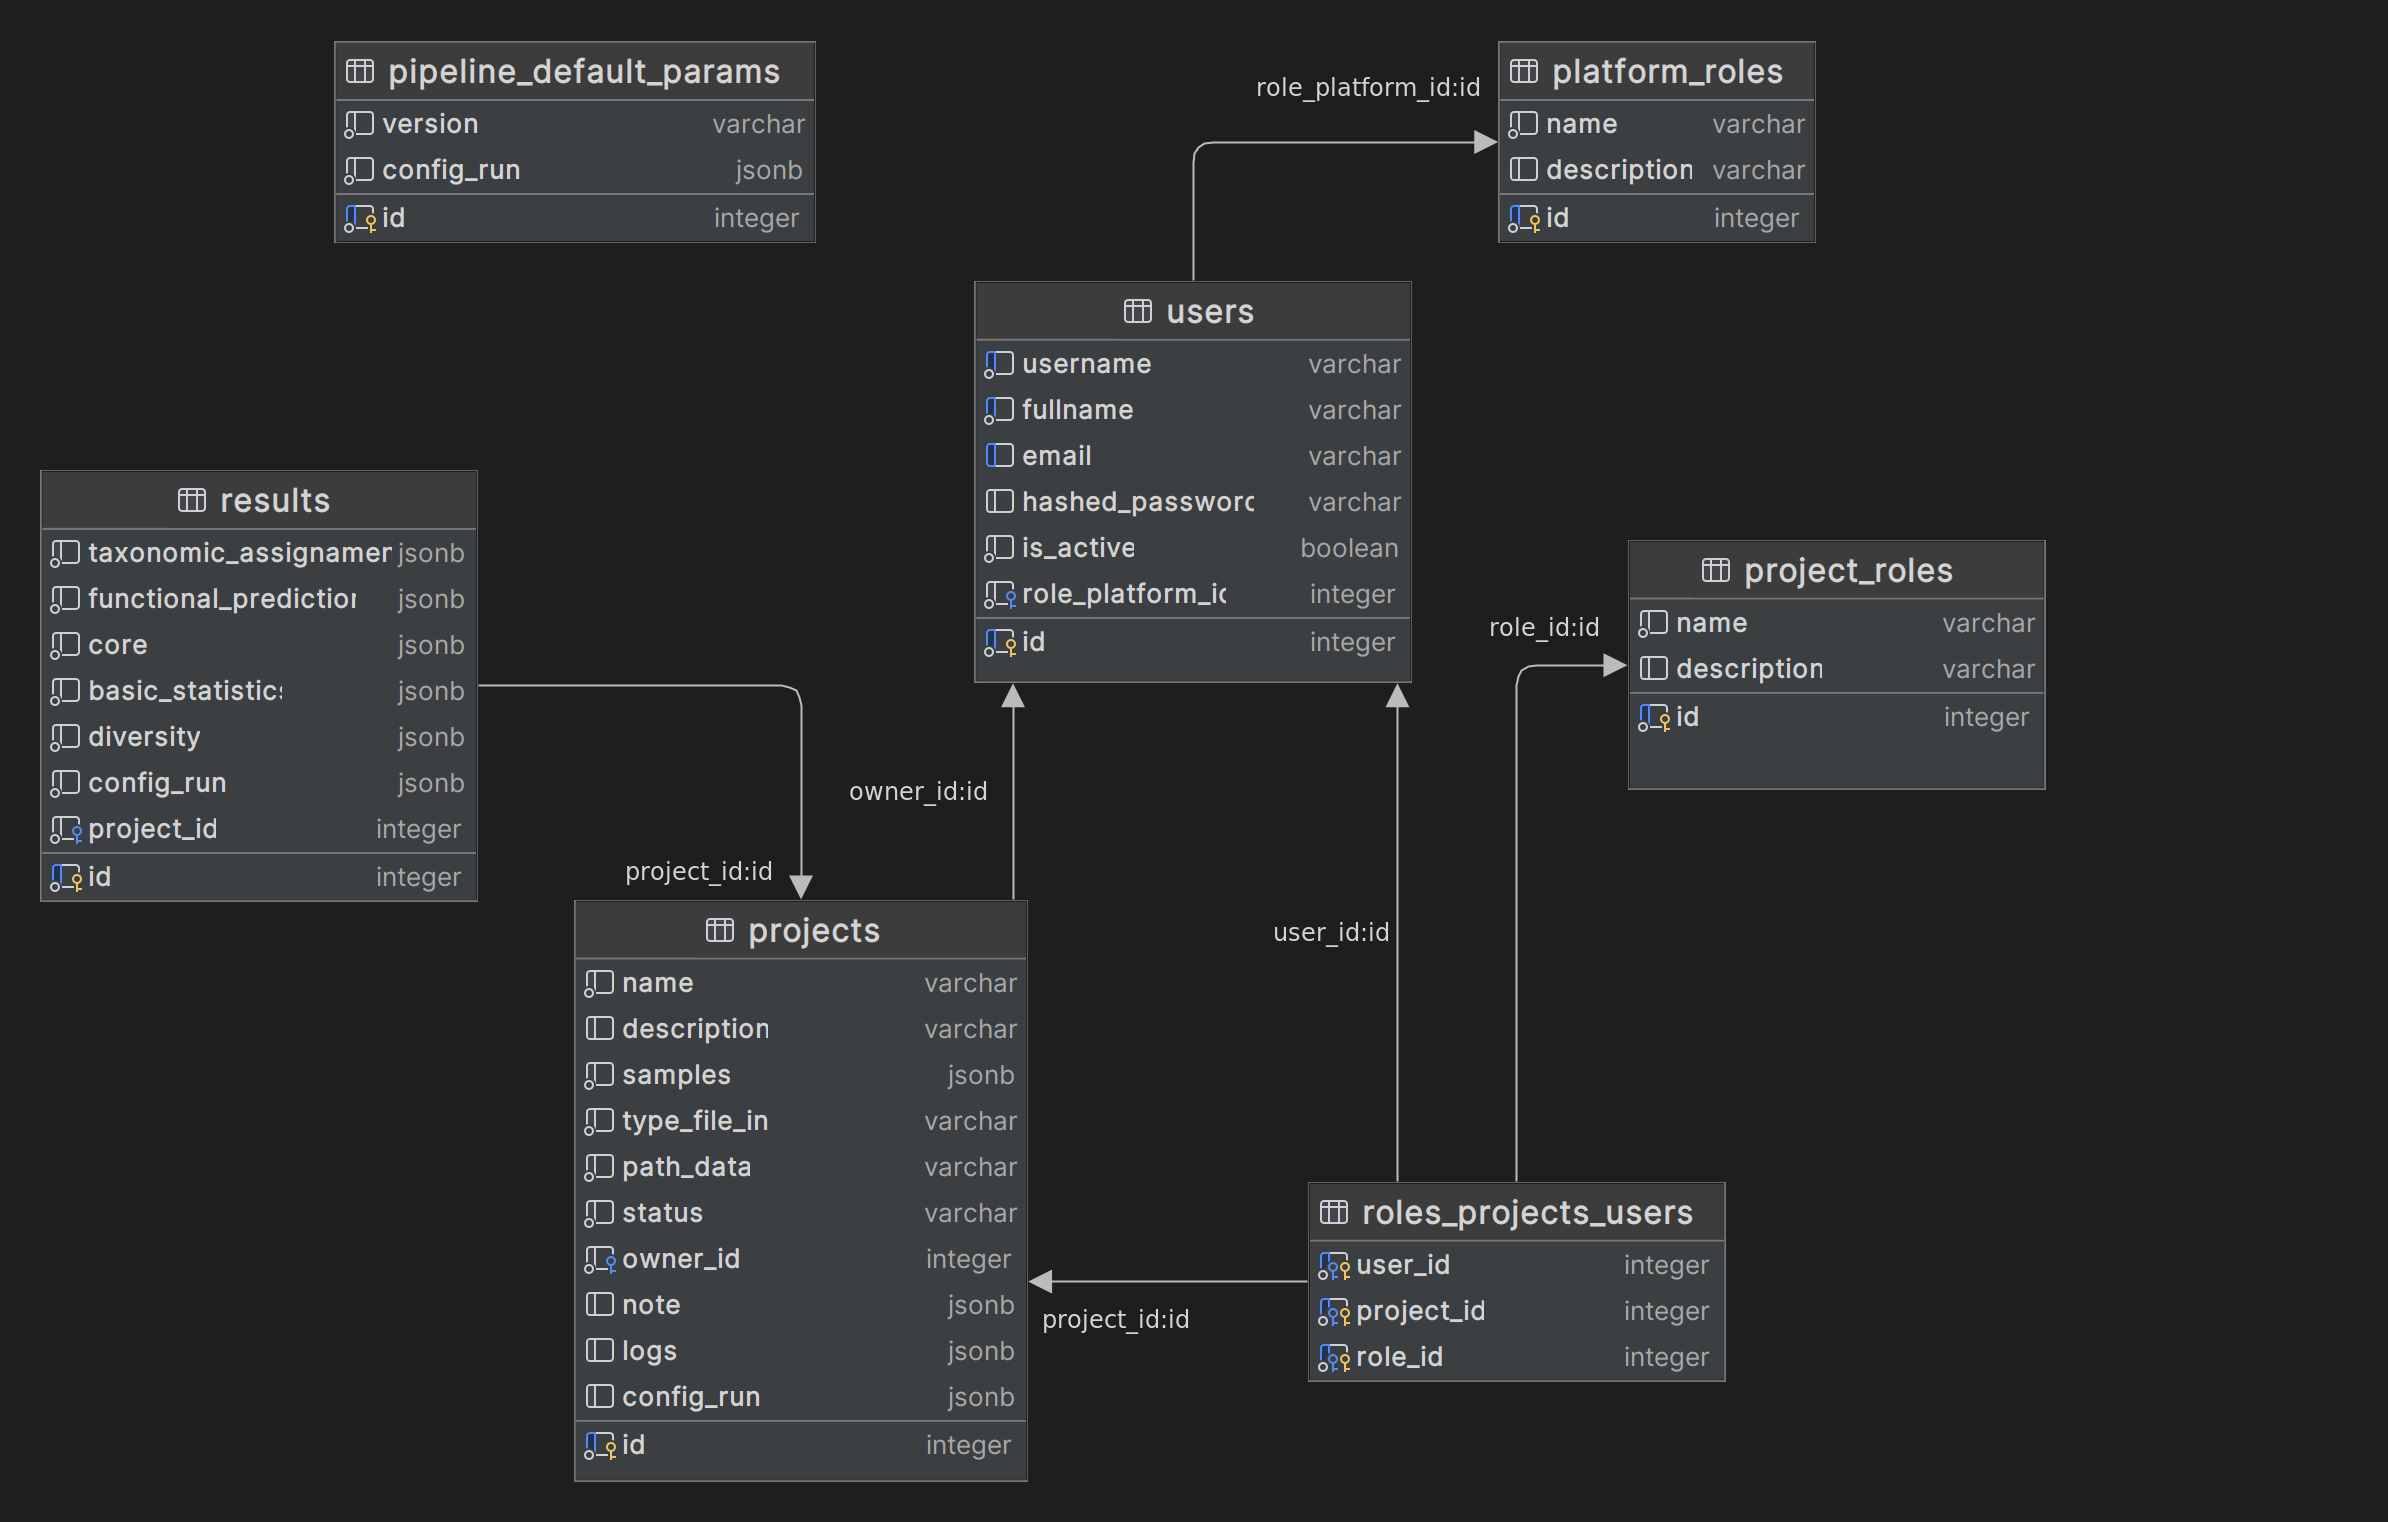
\includegraphics[width=1\linewidth]{images/dbb.png}
    \caption{Base de datos}
    \label{fig:nanotax-db}
\end{figure}

Las tablas de Resultados y Proyectos estan compuestas por campos JSONB que permiten almacenar datos en formato JSON mediante una representación binaria permitiendo que los datos sean indexados y consultados de manera eficiente. 

Para la ejecución del flujo de trabajo se desarrollo un script en Python que escribe el archivo \textit{params.yml} con la información del proyecto y los parámetros ingresados por el usuario en la plataforma (y guardados en la base de datos).
Una vez que el pipeline finaliza su ejecucción mediante un script en Python se almacenan los resultados en la base de datos.

% \subsection{Documentación}
% En esta sección se despliega la documentación del pipeline, la cual cuenta con la información de los módulos, parámetros y herramientas utilizadas en el pipeline. La documentación se encuentra dividida por cada módulo, donde se muestra la versión de la herramienta utilizada y los parámetros por defecto y modificables por el usuario.
% \subsubsection{Basecalling y demultiplexación}
% \subsubsection{Control de calidad}
% \subsubsection{Asignación taxonómica}
% \subsubsection{Predicción funcional}
% \subsubsection{Indices de diversidad}

